%% 
%% Copyright 2007, 2008, 2009 Elsevier Ltd
%% 
%% This file is part of the 'Elsarticle Bundle'.
%% ---------------------------------------------
%% 
%% It may be distributed under the conditions of the LaTeX Project Public
%% License, either version 1.2 of this license or (at your option) any
%% later version.  The latest version of this license is in
%%    http://www.latex-project.org/lppl.txt
%% and version 1.2 or later is part of all distributions of LaTeX
%% version 1999/12/01 or later.
%% 
%% The list of all files belonging to the 'Elsarticle Bundle' is
%% given in the file `manifest.txt'.
%% 

%% Template article for Elsevier's document class `elsarticle'
%% with numbered style bibliographic references
%% SP 2008/03/01

%\documentclass[preprint,12pt]{elsarticle}

%% Use the option review to obtain double line spacing
%% \documentclass[authoryear,preprint,review,12pt]{elsarticle}

%% Use the options 1p,twocolumn; 3p; 3p,twocolumn; 5p; or 5p,twocolumn
%% for a journal layout:
%% \documentclass[final,1p,times]{elsarticle}
%% \documentclass[final,1p,times,twocolumn]{elsarticle}
%% \documentclass[final,3p,times]{elsarticle}
%% \documentclass[final,3p,times,twocolumn]{elsarticle}
 \documentclass[final,5p,times]{elsarticle}
%% \documentclass[final,5p,times,twocolumn]{elsarticle}

%% For including figures, graphicx.sty has been loaded in
%% elsarticle.cls. If you prefer to use the old commands
%% please give \usepackage{epsfig}

%% The amssymb package provides various useful mathematical symbols
\usepackage{amssymb}
%% The amsthm package provides extended theorem environments
%% \usepackage{amsthm}

%% The lineno packages adds line numbers. Start line numbering with
%% \begin{linenumbers}, end it with \end{linenumbers}. Or switch it on
%% for the whole article with \linenumbers.
%% \usepackage{lineno}

\usepackage{algorithm}
\usepackage{algorithmic}

\journal{Parallel Computing}

\begin{document}

\begin{frontmatter}

%% Title, authors and addresses

%% use the tnoteref command within \title for footnotes;
%% use the tnotetext command for theassociated footnote;
%% use the fnref command within \author or \address for footnotes;
%% use the fntext command for theassociated footnote;
%% use the corref command within \author for corresponding author footnotes;
%% use the cortext command for theassociated footnote;
%% use the ead command for the email address,
%% and the form \ead[url] for the home page:
%% \title{Title\tnoteref{label1}}
%% \tnotetext[label1]{}
%% \author{Name\corref{cor1}\fnref{label2}}
%% \ead{email address}
%% \ead[url]{home page}
%% \fntext[label2]{}
%% \cortext[cor1]{}
%% \address{Address\fnref{label3}}
%% \fntext[label3]{}

\title{Improving Data Movement Performance for Sparse Data Patterns on the Blue Gene/Q Supercomputer}

%% use optional labels to link authors explicitly to addresses:
%% \author[label1,label2]{}
%% \address[label1]{}
%% \address[label2]{}

\author[evl]{Huy Bui}
\author[mcs]{Eun-Sung Jung}
\author[mcs]{Venkatram Vishwanath}
\author[evl]{Andrew Johnson}
\author[evl]{Jason Leigh}
\author[alcf,niu]{Michael E. Papka}

\address[evl]{Electronic Visualization Laboratory (EVL), University of Illinois at Chicago, 842 W Taylor St, Chicago, IL 60607, USA}
\address[mcs]{Mathematics and Computer Science, Argonne National Laboratory, 9700 S Cass Ave, Lemont, IL 60439, USA}
\address[alcf]{Argonne Leadership Computing Facility, Argonne National Laboratory, 9700 S Cass Ave, Lemont, IL 60439, IL, USA}
\address[niu]{Northern Illinois University, 300 Normal Road, DeKalb, IL 60115, USA}

\begin{abstract}

In-situ analysis has been proposed as a promising solution to glean faster insight and to reduce the amount of data written out to storage. A critical challenge here is that the reduced dataset needed to visualize a specific region of interest as the simulation is running is typically held on a subset of the nodes and needs to be written out to storage. Coupled multiphysics simulations also produce a sparse data pattern wherein data movement occurs among a subset of nodes. We evaluate the performance of these data patterns and propose several mechanisms for improving performance. Our mechanisms introduce intermediate nodes to implement multiple paths to transfer data on top of default routing algorithms and utilize topology-aware data aggregation to avoid shared bottleneck links. The efficacy of our solutions is evaluated through microbenchmarks and application benchmarks on an IBM Blue Gene/Q system scaling up to 131,072 compute cores. The results show that our algorithms achieve up to a 2X improvement in achievable throughput compared to the default mechanisms.

\end{abstract}

\begin{keyword}
multiple paths \sep sparse data movement \sep topology-aware aggregation \sep data-intensive \sep Blue Gene/Q
%% keywords here, in the form: keyword \sep keyword

%% PACS codes here, in the form: \PACS code \sep code

%% MSC codes here, in the form: \MSC code \sep code
%% or \MSC[2008] code \sep code (2000 is the default)

\end{keyword}

\end{frontmatter}

%% \linenumbers

\section{Introduction}

Data-intensive applications generate large volumes of data. Transferring the data usually burdens the underlying network and storage system. Storage performance is considered to be one of the weakest links in extreme-scale computing. To mitigate this I/O bottleneck, computational science applications use in-situ analysis and visualization wherein the analysis computation is done at simulation time, and a reduced dataset is written out to storage instead of the entire dataset. Such applications produce either evenly-distributed data among the compute nodes, called {\em dense data}, or concentrated data among a partial set of compute nodes, called {\em sparse data}. Several in-situ analyses such as finding regions of turbulence, query-driven analysis, etc., produce sparse data, which needs to be written out to the storage system. Sparse data has a wide distribution of message sizes for I/O across the compute nodes. In many cases, a majority of these nodes, due to the analyses performed, may not have any data to write out to the storage system.

Sparse data is also generated by multiphysics applications wherein we have different physics modules running on disjointed compute partitions. Each module may write out data at differing frequencies, likely non-overlapping, leading to a situation where the entire I/O pipeline may not be utilized to write the data from any single physics module.

Furthermore, sparse data can also be seen in communication between data coupling modules in multiphysics applications when two physics modules communicate while other modules are communication-free. On the IBM Blue Gene/Q system, the data is transferred between the two modules via a single path even though multiple paths are available.. In such cases, the network resources is underutilized and this leads to an increase in the time-to-solution. As we can see more sparse data movements in emerging data-intensive scientific applications, optimizing and improving sparse data transfers are getting more important for those applications.

In this paper, we investigate the performance of sparse data movement on Argonne National Laboratory's IBM BG/Q supercomputer, Mira. More specifically, our contributions are two-fold: 1) we identify sparse data transfer problem in data-intensive applications and develop mechanisms for aggregating data efficiently, and 2) we propose multi-path algorithms leveraging intermediate nodes to improve data transfers among compute nodes. We evaluate the efficacy of the current data movement mechanisms in multiphysics and MPI-IO for sparse data patterns on these systems. We then introduce the intermediate nodes to allow data to be transferred concurrently on multiple data paths at the application level.

We developed heuristics to select the number and position of intermediate nodes to maximize data transfer throughput. We also developed a data movement mechanism that is aware of I/O node location to balance the I/O load. Finally, we evaluate the performance for a set of benchmarks on Mira scaling to 131,072 compute cores.

The remainder of the paper is organized as follows: in Section \ref{sec:relatedwork}, we discuss related work in data movement and I/O performance improvement in high performance systems. In Section \ref{sec:systems} we briefly describe the supercomputing system that we used to investigate our approaches. We present our approaches in Section \ref{sec:approaches} and then demonstrate their efficacy through microbenchmarks in Section \ref{sec:microbenchmarks} and application benchmarks in Section \ref{sec:app_benchmarks}, respectively. Finally, we present our conclusions and future work in Section \ref{sec:conclusions}.

\section{Related work}
\label{sec:relatedwork}

Bandwidth optimization has been studied in great details in the literature. Many works consider a particular system's interconnection information and application's communication patterns to optimize throughput. Essentially, these two characteristics can be used to map an application's processes to specific processors so that interprocessor communication can take advantage of that network.

In an MPI-enabled environment, bandwidth optimization can be done via MPI processes mapping. In \cite{Bhatele:mapping}, the authors provide a tool for performing a wide variety of mappings for structured communication patterns. The tool provided mappings that were able to increase bandwidth and reduce latency and congestion. The tool did not take unstructured communication patterns into account, thus, did not realize that multiple paths could be made available for data movement.

Multiple path data movement was realized in the work of Khanna et al. \cite{Proxies:Gaurav} by using intermediate nodes when an explicit path setup was not provided. This work focused on wide-area networks (WANs) where the exact network topology is hidden from users. Accordingly, shared links are identified through real experimental network throughputs. Our work is applied to the interconnection network and the I/O subsystem of supercomputers where the network topology and associated routing policies are known a priori and the size of the network is much larger than WANs. Our ideas come from the observation that compute nodes in the BG/Q system have 10 links for communication but usually only a single path is used for transferring data between nodes or between nodes and I/O nodes.

Kumar and Faraj \cite{Kumar:Allreduce} proposed using multiple incoming and outgoing links per node for communication on the BG/Q. The work was focused on MPI Allreduce collective communication while our work targets sparse data movement among a subset of nodes.

Adaptive routing for network balancing has also been studied in \cite{Valiant:Routing,singh2003:goal}. In addition, there are works on adaptive routing for current supercomputers such as the BG/Q \cite{Chen:BGQ} and the Cray Cascade \cite{garcia2013:CrayDragonfly}. However, these works are for low-level networking, where any packet can be routed to any path. In contrast, our study leverages underlying routing policies to implement multipath data movement in the user space, where we have more detailed knowledge about the data flows and patterns.

I/O forwarding and staging is routinely used for improving I/O performance to storage. A scalable I/O forwarding framework for high-performance computing systems is presented in \cite{Ali:IOForwarding}. The authors in \cite{Vishwanath:IOForwarding,Vishwanath:GLEAN}  proposed an augmentation for I/O forwarding and asynchronous data staging for BG/P and /Q systems. However, those studies assumed that the data is dense and uniformly distributed. Our work in this paper extends on our previous work \cite{Vishwanath:GLEAN} to deal with sparse data movement patterns.

\section{Supercomputing Systems}
\label{sec:systems}

In this section, we describe the BG/Q resources at the Argonne Leadership Computing Facility (ALCF) on which we developed and tested our multipath sparse data movement algorithms.

ACLF maintains several compute analysis systems that are used by the scientific community. Figure \ref{fig:alcf} depicts the architecture of ALCF’s primary resource, Mira, its data analysis cluster, Tukey, and the file server nodes.

\begin{figure}[!htb]
\vspace{-0.1in}
\centering
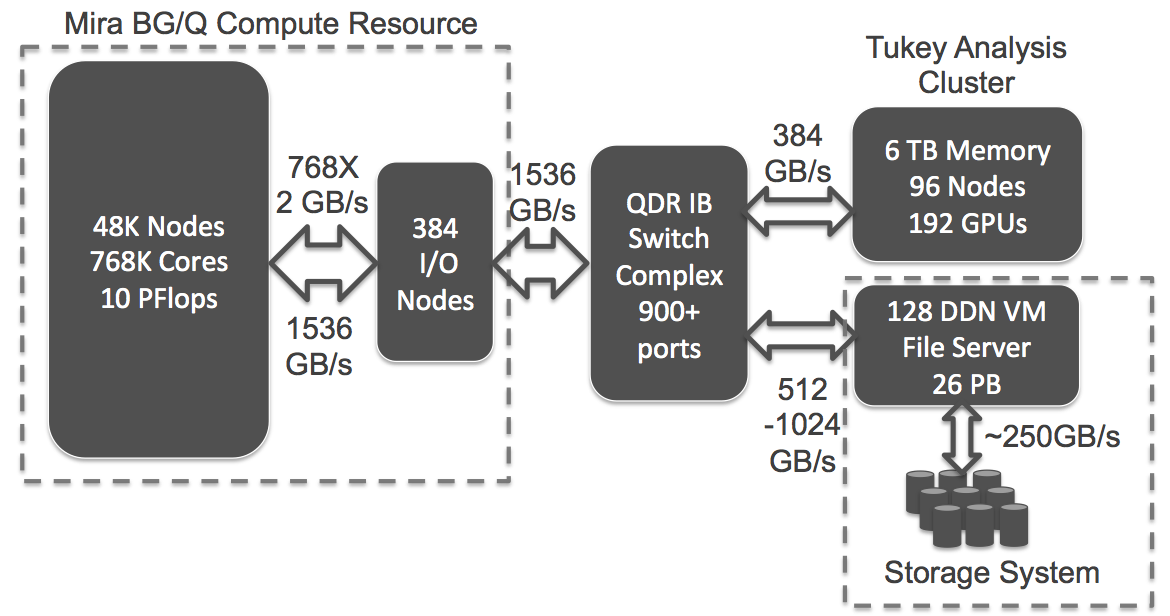
\includegraphics[scale=0.2]{figures/anl_facility}
\vspace{-0.1in}
\caption{The ALCF maintains the 768K core Blue Gene/Q supercomputer (Mira), data analysis cluster (Tukey), and file server nodes.}
\vspace{-0.1in}
\label{fig:alcf}
\end{figure}

Mira has 48K nodes and has a peak performance of 10 petaflops. Each node has 16 application cores and 16 GB of memory.
Mira’s I/O and interprocessor communications (both point-to-point and collectives) travel on a 5D torus network. This 5D torus interconnects each compute node with its 10 neighbors at 2 GB/s theoretical peak over each link in each direction, making a total of 40 GB/s bandwidth in both directions for one single compute node. However, due to packet and protocol overheads, up to 90\% of the raw data rate (1.8GB/s) is available for user data. The machine can be partitioned into non-overlapping rectangular sub-machines for certain applications upon request. These sub-machines do not interfere with each other except for I/O nodes and the corresponding storage system.

An overview of the network is also given in \cite{Chen:MessagingUnit}. Each compute node has 11 send units and 11 receive units (10 for the links of the torus and one for the I/O link). All packets are injected in and pulled out of network injection/reception FIFOs by Messaging Unit (MU). The number of FIFOs is enough to saturate all links. Outgoing packets can be put in any injection FIFOs and may go out to any link. However, incoming packets at a receiver is placed only in its reception FIFO.

For interconnect network traffic, the BG/Q supports both deterministic and dynamic routing \cite{Chen:BGQ}. Deterministic routing uses only one path to route packets from a source to a destination and packets are routed longest to shortest using a commonly used dimension-order routing algorithm. In dynamic routing, routing is still dimension ordered, but the packet routes are programmable, enabling different routing algorithms to be used. This is called ``zone routing''. There are four zone IDs from 0 to 3. The routing algorithm selects a zone ID based on a flexibility metric and the message size. The flexibility value is computed based on the torus size and hop distance between the two communicating nodes. The selection of zone ID based on these values is experiment-based and is hard coded in low-level libraries \cite{BGQRedbook:Gilge}. Among the four routing zones, routing zone ID 1 is unrestricted, and packets route in a random order. Routing zone ID 0 is longest-to-shortest. However, dimensions with the same lengths can be chosen randomly. Routing zone IDs 2 and 3 are deterministic. For these two routing zone IDs, given a certain message size, routing is always the same and its path is known before it is routed. These are default routing algorithms and are not changeable. However, we can set a routing zone ID by using a PAMI ROUTING environment variable. As BG/Q uses single path data routing, only one of ten available links are used for message sending and receiving a message, so one reception FIFO is used at receiver.

With respect to I/O traffic, the compute nodes connect to an analysis cluster and the file servers through I/O nodes and a QDR IB Switch Complex. Every 128 compute nodes (forming a pset) has two bridge nodes, which are among the compute nodes. Each bridge node has an 11th 2GB/s-bandwidth link connecting to an I/O node, making total 4 GB/s bandwidth for I/O per pset at most. I/O traffic is routed from compute nodes to bridge nodes over the torus network deterministically, and then traverses over the 11th links from bridge nodes to the I/O nodes \cite{Chen:BGQInterconnection}. In the next section, we describe novel multipath routing mechanisms that leverage default routings on the BG/Q to improve data movement performance.

\section{Sparse data movement optimization}
\label{sec:approaches}
We start this section by presenting inefficiencies in current systems in the support of sparse data movement. We propose novel approaches for multipath data movement to overcome these inefficiencies.

\subsection{Inefficiency in current data movements}
For data transfers between compute nodes on the BG/Q, a message from a source to a destination traverses a single path. In the absence of congestion and network failures, default routing algorithms are used, causing the message to traverse a deterministic and single path. Figure \ref{fig:multiply}(a) depicts the single path data movement, in which one path is used other paths are idle. With dense, uniform data movement patterns where a majority of nodes and network links are involved in communications, the utilization of system resources is high. Whereas with sparse data movement patterns, only specific regions of the system are involved in communications, resulting in a low utilization of the resources.

Similarly, I/O messages such as writes as shown in Figure \ref{fig:multiply}(b) travel along a default path to default I/O nodes. When the writes  have a uniform distribution on data size and location, I/O nodes allocated for applications are used efficiently. However in sparse data movements, due to uneven distribution of data movement requests, I/O nodes and the interconnect networks suffer from an unbalanced load. The current MPI-IO implementation aggregates data to intermediate nodes, but these nodes are neither uniformly distributed nor balanced to connect to all I/O nodes. 

We next present a general approach to improve resource utilization for data movement. We then present two sub-algorithms for sparse data movements, one for among compute nodes and the other for between compute nodes and I/O nodes.

\subsection{Data movement using multiple paths}
One way to improve the utilization is to employ multiple paths. We can assign non-overlapping multiple paths for multiple messages going out from a node. Theoretically, each message would concurrently follow a non-overlapping path and the data movement therefore promises to achieve  improvement. However, at programming level, the current BG/Q system has no ability to set up paths for messages explicitly. However, we can still leverage disclosed default routing algorithms to implement concurrent data movement via multiple paths in the user-space. Thus, we can greatly simplify the deployment of our heuristics.

\begin{figure}[!htb]
\vspace{-0.1in}
\centering
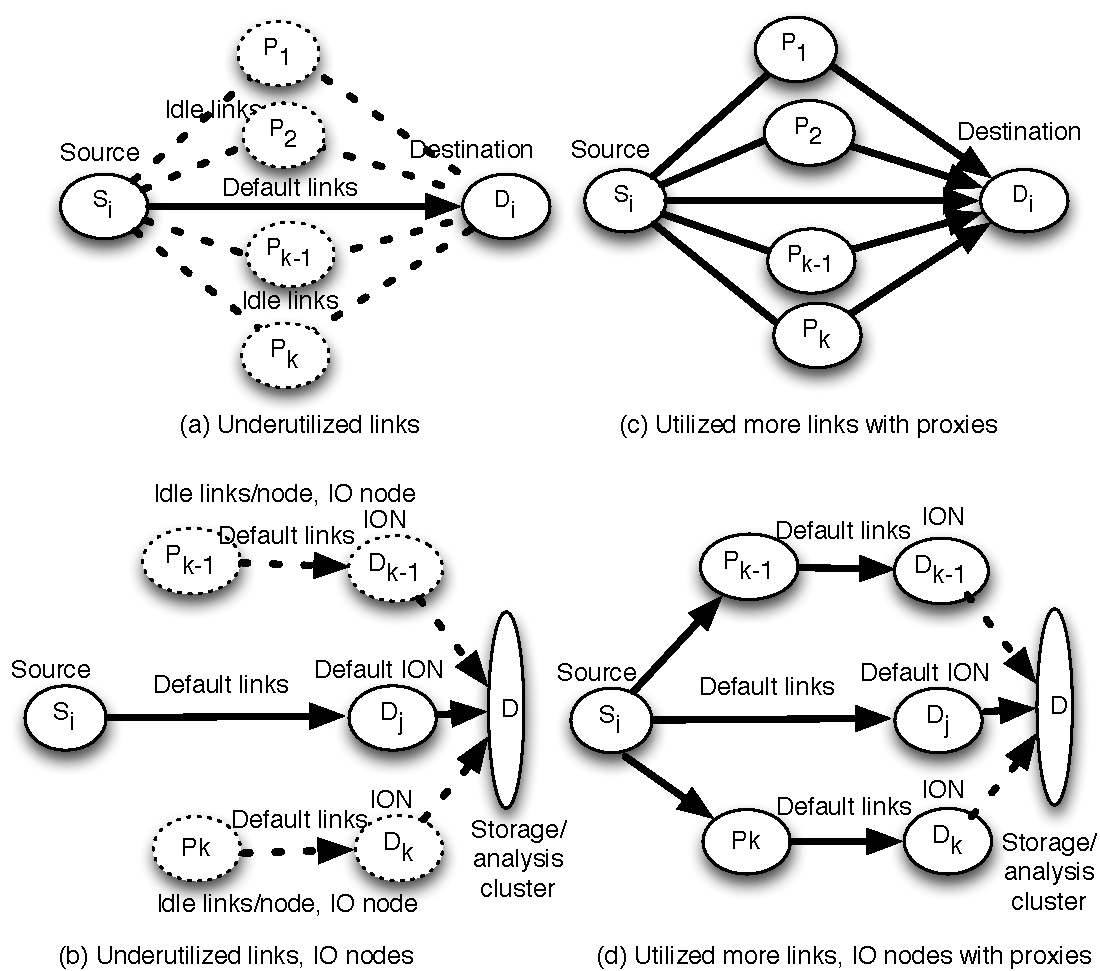
\includegraphics[scale=0.5]{figures/multiply}
\vspace{-0.2in}
\caption{Data transfer with and without proxies}
\vspace{-0.1in}
\label{fig:multiply}
\end{figure}

In order to route data along multiple paths on a single-path-allowed system, we introduce intermediate nodes which are compute nodes where the application runs to serve an additional purpose of routing data. Leveraging the default routing, we first route data from sources to the intermediate nodes and then from intermediate nodes to destinations. As shown in Figure \ref{fig:multiply}(c), by adding intermediate nodes we increase the number of paths to move data between nodes, overcoming the system limitation of a deterministic single path for data movement. The  routing function on the intermediate nodes does introduce little additional overheads, and we assume that future systems might provide such functionality at the node level for a multipath routing.  Knowing the routing policy a priori, we choose the locations of intermediate nodes to minimize the shared links and therefore maximize the data movement throughput. In Figure \ref{fig:multiply}(d), by adding the intermediate nodes we increase the number of I/O nodes and accordingly balance I/O workload. 
We also propose a mechanism that leverages interconnect topology and distributes intermediate nodes dynamically among all I/O nodes to achieve significant improvement in I/O. 

Implementing multipath data movement using intermediate nodes requires several steps.
\begin{itemize}
\item Calculate the message sizes to see if using intermediate nodes benefits performance and how to use them.
\item Determine the number and location of intermediate nodes.
\item Transfer data using multipaths from sources to destinations via intermediate nodes.
\end{itemize}

In the next sections, we realize the above steps for sparse data movement among compute nodes and sparse data movement to I/O.

\subsection{Sparse data movement between groups of compute nodes}
In this subsection, we present an algorithm to select the number and the locations of intermediate nodes together with multipath data movement between two groups of compute nodes. This is critical for data coupling in multiphysics codes. Intermediate nodes will be referred to as proxies for the rest of the paper. 

We start with selecting number of proxies. Each proxy adds an additional non-overlapping data movement path,. Adding more paths reduces congestion and improves the transfer time. However, as we introduce proxies, additional overhead, and hence time, is also introduced due to the additional processing and buffering at the proxy. Therefore performance gained by introducing proxies needs to be at least enough to compensate the extra time caused by introducing them. We model the time for data movement from one node's memory to another node's memory using remote direct memory access (RDMA) as follows.

\begin{figure}[!htb]
\vspace{-0.1in}
\centering
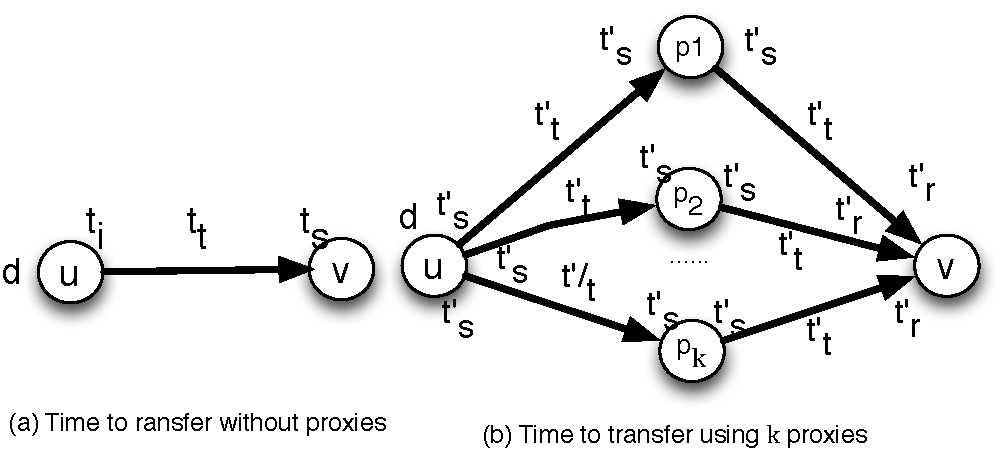
\includegraphics[scale=0.5]{figures/transfer_time.pdf}
\vspace{-0.2in}
\caption{Time to transfer in case of with and w/o proxies}
\vspace{-0.1in}
\label{fig:proxies}
\end{figure}
For data transfer, communication delay is composed of processing delay, transmission delay, queueing delay and propagation delay. To make it simple, we model the delays into 3 variables: time for processing, queueing and injecting at sender node t$_s$, time to transfer data t$_t$ and time for processing, queueing and storing at receiver node t$_r$. The time is depicted in Figure \ref{fig:proxies}. The total time to transfer a message of size d from sender u to receiver v therefore is:

\begin{equation}
t = t_s + t_t + t_r
\end{equation}

In which:
\begin{itemize}
\item $t$: Total time to transfer.
\item $t_s$: Time to process, queue and inject a message of size d into the network at sender
\item $t_t$: Time to actually transfer a message of size d from sender' network interface to receiver's network interface.
\item $t_r$: Time to process, queue and store a message of size $d$ from network to memory at receiver.
\end{itemize}

In the case of using k paths with k proxies, the data size each path carries would be $\frac{d}{k}$, assuming equal split. Data is transferred in two steps from the sender to proxies, completely stored at the proxies, and then moved from the proxies to the receiver. Each proxy becomes an extra sender and receiver. Thus, we need to account for this additional processing and buffering at proxy endpoints. The time for transfer in each hop can be considered approximately the same. Hence, total time to transfer data is:
\begin{equation}
t' = 2(t'_s + t'_t + t'_r) %2(\frac{t'_i}{k} + \frac{t'_t}{k} + \frac{t'_s}{k}) = 2\frac{t'_i + t'_t + t'_s}{k}
\end{equation}

In which:
\begin{itemize}
\item $t'$: Total time to transfer.
\item $t'_s$: Time to process, queue and inject a message of size d/k into the network at sender
\item $t'_t$: Time to actually transfer a message of size d/k from sender's network interface to receiver's network interface.
\item $t'_r$: Time to process, queue and store a message of size d/k from network to memory at receiver.
\end{itemize}

The ratio of total time for two data transfer methods is:
\begin{equation}
\frac{t'}{t} = \frac{2(t'_s + t'_t + t'_r)}{t_s + t_t + t_r} 
\end{equation}

As we split a message into k messages, time to transfer data is reduced linearly. However, the time to inject and  to store do not. Actually the total time to inject or store $k$ messages of size d/k each is at least the time for one single message size $d$. This is due to overheads to process and buffer the data. Therefore:

\begin{equation}
t'_s \ge \frac{t_s}{k}; \; 
t'_t = \frac{t_t}{k}; \; 
t'_r \ge \frac{t_r}{k}\; 
\end{equation}

The equalities happen only when message size is greater than a threshold. For the message size greater than  the threshold, we have:
\begin{equation}
\frac{t'}{t} = \frac{2(t'_s + t'_t + t'_r)}{t_s + t_t + t_r} = \frac{2(\frac{t_s}{k} + \frac{t_t}{k} + \frac{t_r}{k})}{t_s + t_t + t_r} = \frac{2}{k}
\end{equation}

Thus, to get benefit from setting up proxies, we need to have at least 3 proxies per data transfer, and we can improve $k/2$ times throughput.

For small messages, as $t'_s \gg t_s/k$ and $t'_r t_r/k$, we need a much greater value of k to get benefit from setting up proxies, which is usually not feasible. In Section \ref{sec:microbenchmarks}, we show threshold values computed based on experiments at which for smaller messages, direct transfer is better than proxy-based transfer, and for bigger messages, proxy-based transfer is better. Therefore, proxy-based techniques should be used for intensive sparse data movements when the size of message is greater than a threshold.

With respect to the placement of the proxies, we need to choose positions of the proxies to minimize link sharing since we know routing paths in advance. It is difficult and sometimes impossible to choose proxies as the number of nodes involved in data movement increases. We develop an heuristic algorithm to check if it is feasible to implement proxies and to find the number and position of these proxies. The BG/Q is connected via 5D torus, however to simplify the algorithm illustration and description, we depict the data movement of the algorithm for 2D mesh as in Figure \ref{fig:groxies}. The 5D torus or any k-D torus would work in the same way. In our work, we assume that regions of a cluster that need to communicate data are contiguous. This assumption is valid under many multi-physics applications such as Community Earth System Model \cite{CESM:Collins} as processes of an application are usually mapped contiguously to improve intra-group communication. We also assume that the network is dedicated with no background communication from other applications.

\begin{figure}[!htb]
\vspace{-0.1in}
\centering
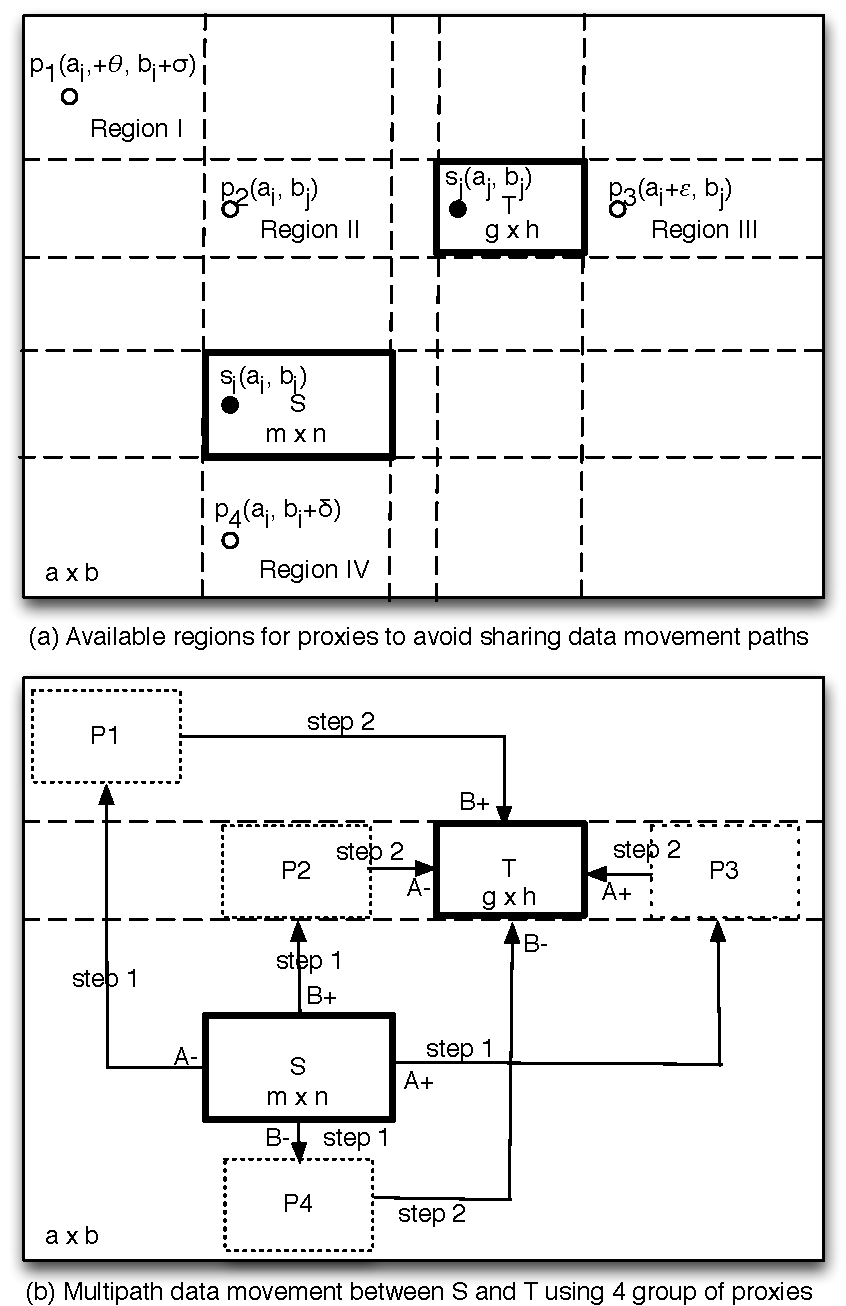
\includegraphics[scale=0.5]{figures/groxies.pdf}
\vspace{-0.1in}
\caption{Using 4 groups of proxies at 4 directions to transfer data between 2 groups in 2 steps}
\vspace{-0.2in}
\label{fig:groxies}
\end{figure}

The Figure \ref{fig:groxies} depicts a 2D allocation of \textit{a} x \textit{b} mesh topology for multi-physics application. In the 2D mesh, data is routed horizontally (A direction) first and then vertically (B direction). Two physics codes S and T running at 2 regions of the cluster are data coupled (i.e., T needs data from S to complete a computation.) Region S has the size \textit{m} x \textit{n}, while T has the size \textit{g} x \textit{h}. We assume that each node has approximately the same amount of data and each destination receives approximately the same amount of data.

\begin{itemize}
\item S: Set of source nodes, size $|S|$ = m*n = M
\item T: Set of destination nodes, size $|T|$ = g*h = N
\item P$_i$: Proxies nodes of source node s$_i$.
\item L: Number of dimensions of the network.
\item $coord_{il}$: Coordinate of a node i, dimension l
\item Each s$_i$ $\in$ S:
\begin{itemize}
\item Has targets T$_i$ and proxies P$_i$.
\item Data size d$_i$ at s$_i$ is sent to set of t$_i$ in T$_i$. s$_i$ sends d$_{i}$ to t$_i$ through p$_i$

\end{itemize}
\end{itemize}

Here we develop a heuristic algorithm for data movement between multiple sources and multiple destinations using multiple paths leveraging known  data routing algorithms. Note that the default routing algorithms here is order-based and given the torus size of the allocation, message size and coordinates of source and destination are known a priori. The algorithm is described in Algorithm \ref{Alg:groxies}.

\begin{algorithm}
\caption{Algorithm for data movement between 2 groups of nodes}
\begin{algorithmic}

\STATE \textbf{I. Init}
\STATE Exchange coordinations of the sources and destinations.
\FOR {each node s$_i$ in S with i = 1..M}
\STATE P$_i$ = $\varnothing$, T$_i$ = $\varnothing$.
\STATE Adding its destination nodes t$_j$ into T$_i$.
\ENDFOR

\STATE \textbf{II. Find Proxies}
\FOR {each source node s$_i(\{coord_{il}\})$ in S}
\FOR {each its destination node $t_j({coord_{jl}})$ in T$_i$}
\STATE Sort the dimensions by routing order.
\FOR{each dimension l with l = 1..L in the sorted order}
\STATE Check 2 candidates: c$_p$ and c$_n$ on the + and - on the l direction of the s$_i$. %$(a_i, b_j), (a_i+\epsilon, b_j), (a_i, b_i+\delta), (a_i+\theta, b_i+\sigma$) w.r.t $(a_j-a_i)*(a_j-(a_i+\epsilon)) < 0, (b_i-b_j)*(b_i-(b_i+\delta)) < 0, (b_j-b_i)*(b_j-(b_i+\sigma)) < 0, (a_i-a_j)*(a_i-(a_i+\theta)) < 0$.
\STATE If a candidate is available, add it into P$_i$.
\ENDFOR
\ENDFOR
\IF {$|Pi| < 3$} \STATE Exit. \ENDIF
\ENDFOR

\STATE \textbf{III. Multipath Data Movement}
\STATE Phase 1: At each node s$_i$ in S:
\FOR{\textbf{each} p$_{ij}$ in P$_i$}
\STATE Send data to p$_{ij}$ with size d$_{ij}$.
\ENDFOR
\STATE Phase 2: At each proxy p$_{ij}$:
\STATE Send data to the destination.
\end{algorithmic}
\label{Alg:groxies}
\end{algorithm}

Our algorithm includes 3 parts: In the \textbf{Init} part, we exchange the coordinates of all sources and destinations. After that, each node s$_i$ initializes its empty sets of proxies P$_i$ and destinations T$_i$. The destinations of s$_i$ are then added to the T$_i$. If the set of sources and destinations are known a priori, an application only needs to run \textbf{Init} once. In the \textbf{Find Proxies} part, each source node checks 2*L possible candidates along L destinations. In the 2-dimension mesh, each node has 4 directions of +A, -A, +B and -B to send/receive data. There are 4 regions marked from I to IV in Figure \ref{fig:groxies}(a) to search for possible proxies that guarantee non-overlapping concurrent data movements. We can search for 4 proxies in the 4 regions with offsets from the source and the destination represented by values of $\epsilon, \delta, \theta, \sigma$. This is to make sure that 4 proxies are in the 4 distinct directions for both outgoing and incoming transfers.  Due to small torus size, searching for these values are not time consuming. If those values exist, we then add the proxies into the list P$_i$. If each source node can have at least 3 proxies then we continue the next part. Otherwise, we discard since there is no benefit to setup proxies. In the last part, \textbf{Multipath Data Movement}, we first move data from source nodes to proxies and then from proxies to destination nodes. To extend for L dimensions, we need to search for 2L directions (both negative and positive directions per each dimension) to find at most 2L proxies.

The algorithm is distributed and runs at every node. Except for gathering all coordinates at the beginning, the remainder of the algorithm executes without waiting (synchronizing) for all other nodes. The running time of the algorithm is O(M*N*L). However, due to small sizes of most networks, the actual time to compute the routes is small. Overall, the overhead for searching for proxies is negligible.

\subsection{Sparse data movement between compute nodes and I/O nodes}
\label{sec:stagingandio}
Each compute node is associated with a default I/O node. Therefore, we need to have at least one intermediate node for each I/O node available in the allocated partition to use the I/O node.
Depending on the data size, we may need more than one intermediate node per I/O node. Also, these intermediate nodes need to be uniformly distributed to avoid data congestion when sending data from compute nodes to intermediate nodes. Thus, to calculate the number of intermediate nodes needed, we need to know total size of data, available I/O nodes, location of compute nodes and their default I/O node. We uniformly distribute these intermediate nodes to the I/O nodes. Data is then aggregated from compute nodes to these intermediate nodes. In this way, an I/O node for which all of its compute nodes do not have data or have small size of data still receives I/O requests with approximately equal amount of data as intermediate nodes are chosen among its compute nodes. As these intermediate nodes aggregate data from a large number of nodes, we call them aggregators. The approach is presented in Algorithm \ref{Alg:aggregation}.

\begin{algorithm}
\caption{Algorithm for I/O data movement}
\begin{algorithmic}
\STATE \textbf{I. Init}
\STATE Define the smallest size of data aggregated at each aggregator S.
\STATE Each node queries its coordinates and its default I/O node.
\STATE Calculate total number of IO nodes for the partition: n$_{io}$.
\STATE List number of aggregators may be needed per I/O nodes: P = \{1,2,4..., 128\}.
\FOR {each value num\_agg in the list P}
\STATE Calculate the positions of aggregators based on the number of aggregators (num\_agg):
\STATE Divide the pset along 5 dimensions by factors nA, nB, nC, nD, nE such as nA*nB*nC*nD*nE = num\_agg to create blocks.
\STATE For each block, choose the first one as the aggregator.
\STATE Save the aggregators for later use.
\ENDFOR

\STATE \textbf{II. Redistribute data}
\STATE Reduce and broadcast the total size of data need to be written: T = $\sum_{i=1}^{n}d_i$.
\STATE Calculate the number of aggregators needed per pset: num\_agg = T/S/n$_{io}$.
\STATE Based on num\_agg select the list of the aggregators from pre-created list and broadcast it to nodes having data.
\STATE Each nodes having data sends its data to its chosen aggregator(s).
\STATE Selected aggregators send data out through I/O nodes.
\end{algorithmic}
\label{Alg:aggregation}
\end{algorithm}

In the first part of the algorithm, \textbf{Init}, the algorithm queries all the information of I/O nodes, coordinates of compute nodes and its default I/O node. It then precomputes all possible aggregators and their location at all processes. The data is stored in list P, used later for redistributing data. To compute P, it divides the partition into equal blocks. It can create a subcomm using MPI\_Comm\_create for each sub-network and select the MPI rank 0 of the subcomm as the aggregator of the subnetwork. In the second part, \textbf{Redistribute data}, depending on total size of data for each I/O request, it selects appropriate aggregators and then carries multipath data movement.

Since all the necessary information is queried and computed once at the beginning, we save time at each I/O request. At each I/O request, the only information needed to gather is total size of data. The aggregators are chosen dynamically and distributed uniformly to balance the load among I/O nodes.

\subsection{Pipeline technique for data movement}
In the graph model, data is transferred from a source to destination through proxies without extra delay. As we have to transfer data from the source node to proxies first, then from the proxies to the destination, we need to store data at a proxy. If we store entire message at the proxy, it takes time to wait until the entire message arrives and  then start injecting the message into network to the next proxy. To reduce the time to wait, we cut the message into smaller messages and transfer messages using pipeline such that storing messages and sending messages at a proxy can run concurrently. %Figure \ref{} depicts the process.

%\begin{figure}[!htb]
%\centering
%\includegraphics[scale=0.5]{figures/pipeline.pdf}
%\caption{Using pipelining technique to eliminate the waiting time at proxy}
%\label{fig:pipeline}
%\end{figure}

For each proxy, requests to wait for data is posted at the beginning. After that, the proxy needs to iterate through the list of requests while checking if data is ready to forward. To implement the pipeline, we create two threads at each proxy: one thread for receiving data and the other for forwarding data. A message is cut into smaller message with certain size called window size. The size of window depends on message size and is determined based on experiments. Within each message we embed the information of how data would be process at the next node such as destination, address of the message in the destination's buffer, the path Id that next node should use to forward the message. The pipeline technique can be used in any system and yields significant improvement as we show in section \ref{sec:microbenchmark}. However, with small messages, we still suffer performance degradation. This is because the control overhead in small message is significantly large compared to the message size itself.

In the following sections, we present our study on Mira Blue Gene/Q to show the efficacy of our solutions.

\section{Microbenchmarks}
\label{sec:microbenchmarks}
In this section, we show the efficacy of our solutions through a set of microbenchmarks for 2 cases: data movement for data coupling nodes and data movement between compute nodes and I/O.

\subsection{Efficacy of proxies and pipeline technique}

%On BG/Q, we tested the system with 16 cores per node all communicate with 16 cores on another node, they transferred in all same links, resulting in 1.7GB/s at most. Due to the symmetry of mapping, it's more likely to all cores belonging to a nodes to connect with all cores belonging another nodes than connect with cores at different nodes. With 20 links per nodes, using multiple paths for data movement on BG/Q can results in significant throughput improvement. 

In this microbenchmark, we transfer data between two nodes through an intermediate nodes using pipelining and compare results with transferring data without using pipeline and with a direct transfer (default) scheme. We varied the data size from 1K  to 128MB.

\begin{figure}[!htb]
\centering
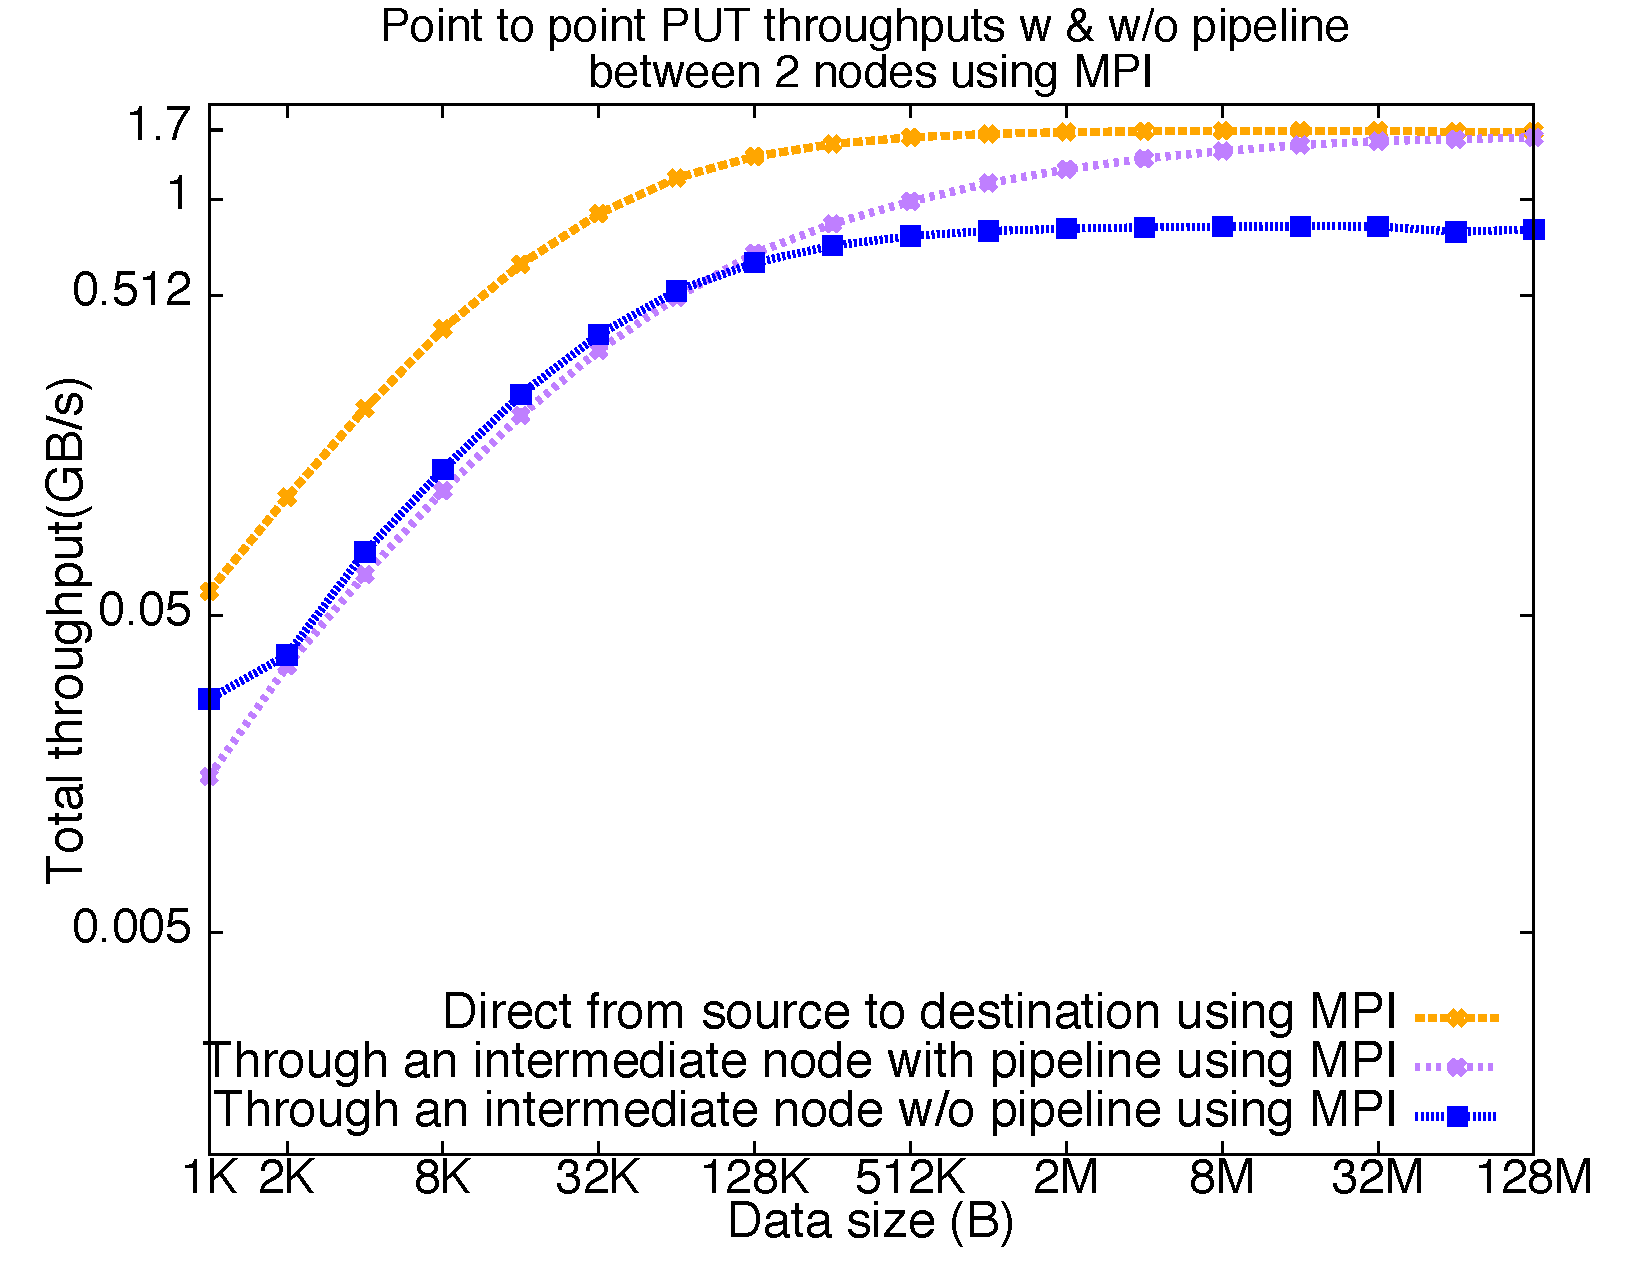
\includegraphics[scale=0.3]{figures/pipeline_mpi.pdf}
\caption{Using pipelining technique to mitigate the waiting time at proxy nodes}
\label{fig:pipeline_mpi}
\end{figure}

Fig. \ref{fig:pipeline_mpi} shows that transferring data through a proxy without using pipelining results a 50\% hit in performance over a direct transfer. This is because the proxy needs to wait until entire data is ready before forwarding it to the destination. By using pipelining, for message less than 64KB,  pipelining does not improve performance, however, for a message size larger than 64KB, pipelining demonstrates an improve performance. At a  message size of 1MB, 2MB, and 4MB, we achieve 70\%, 80\%, and  90\% respectively of the direct transfer bandwidth, and with larger size messages, we achieved a similar performance. Thus, with large size messages, pipelining technique can be used to transfer data through proxies. However, with small size messages, the performance gained is insignificant. Much of the performance overhead is due to the underlying rendezvous protocol design in MPI on the BG/Q. Next, we use PAMI to improve the performance for small messages. The next subsection, we show the efficacy of using PAMI on transferring small size messages.

\subsection{Quantifying computation used for data movement at proxies}
In this section, we quantify the time spent by the CPU for data movement, and we show that it is so small that it has no effect on the total time.

\subsection{Data movement for data coupling nodes}
In this benchmark, we show feasibility of the approach using proxies to increase transfer throughput between 2 compute nodes. We choose the first and the last node of a partition of 128 compute nodes with 2x2x4x4x2 torus. As the partition is large enough we are able to choose 4 proxies to transfer data in 4 directions +B, +C, +D, +E . In each node, only one MPI rank is used (when we use multiple MPI ranks per node to send data to the same destination, they all take the same output link, thus using one MPI rank is still valid and making the experiment easier). The data is transferred in increasing size from 1KB up to 128MB of data, with the size doubled each time. We use MPI\_Put to transfer data from source node to proxy nodes and then from proxy nodes to destination node. Each transfer is repeated multiple times with different data to eliminate any cache effect and achieve stable performance. The average transfer throughput between 2 nodes is reported in Figure \ref{fig:4proxies}.

\begin{figure}[!htb]
\vspace{-0.1in}
\centering
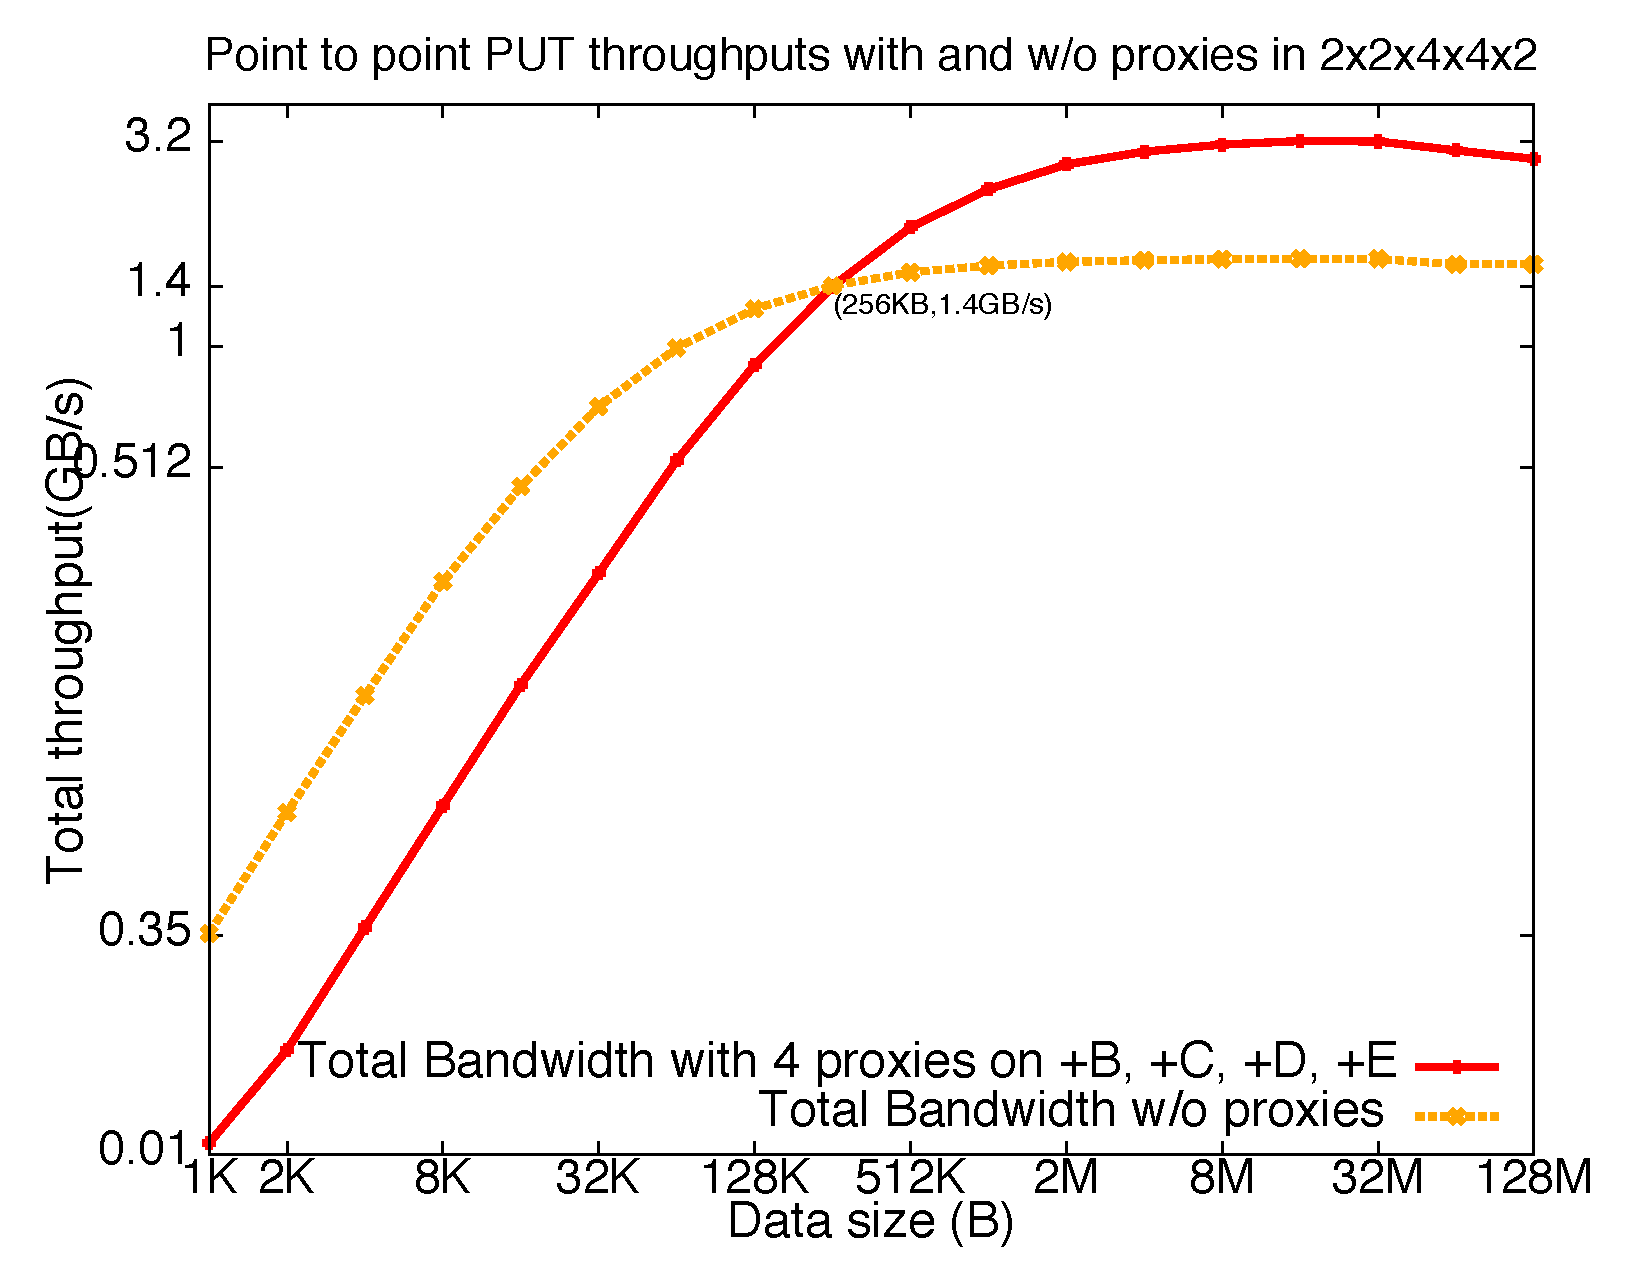
\includegraphics[scale=0.3]{figures/4proxies}
\vspace{-0.2in}
\caption{Using 4 proxies to improve data transfer throughput between 2 nodes}
\vspace{-0.1in}
\label{fig:4proxies}
\end{figure}

As the figure shows, for the small messages, direct transfer yields better performance. With large message, proxy-based transfers outruns direct transfer with $2\times$ better performance. This is foreseen with the reasons we mentioned before: with small messages, extra time caused by injecting and copying messages is significantly larger than the transferring time. It happens in the opposite way with large messages. The message size threshold to switch from direction transfer to proxy-based transfer is 256KB, yielding 1.4GB/s per link. After the threshold, direct transfer slowly reaches to maximum ~1.6BG/s while proxy-based transfer continue to thrive until ~3.2GB/s. Thus, the benchmark shows that proxy-based approach is feasible and can result significant improvement.

As data movement in multiphysics applications is done by more than 2 single nodes, the second benchmark elucidates the feasibility and achievable throughput for data movement between two groups of nodes. In this experiment, we transfer data between two groups of nodes, wherein each group has 256 nodes in a 4x4x4x16x2 torus of a 2K nodes partition. One group is at one corner of the partition, the other one is at the other end of the partition. The data size is also from 1KB to 128MB with doubled size each step. The experiment is repeated for a number of times. We are able to choose 3 proxies for each node. The Figure \ref{fig:3groxies} shows the average throughput measured.

\begin{figure}[!htb]
\vspace{-0.1in}
\centering
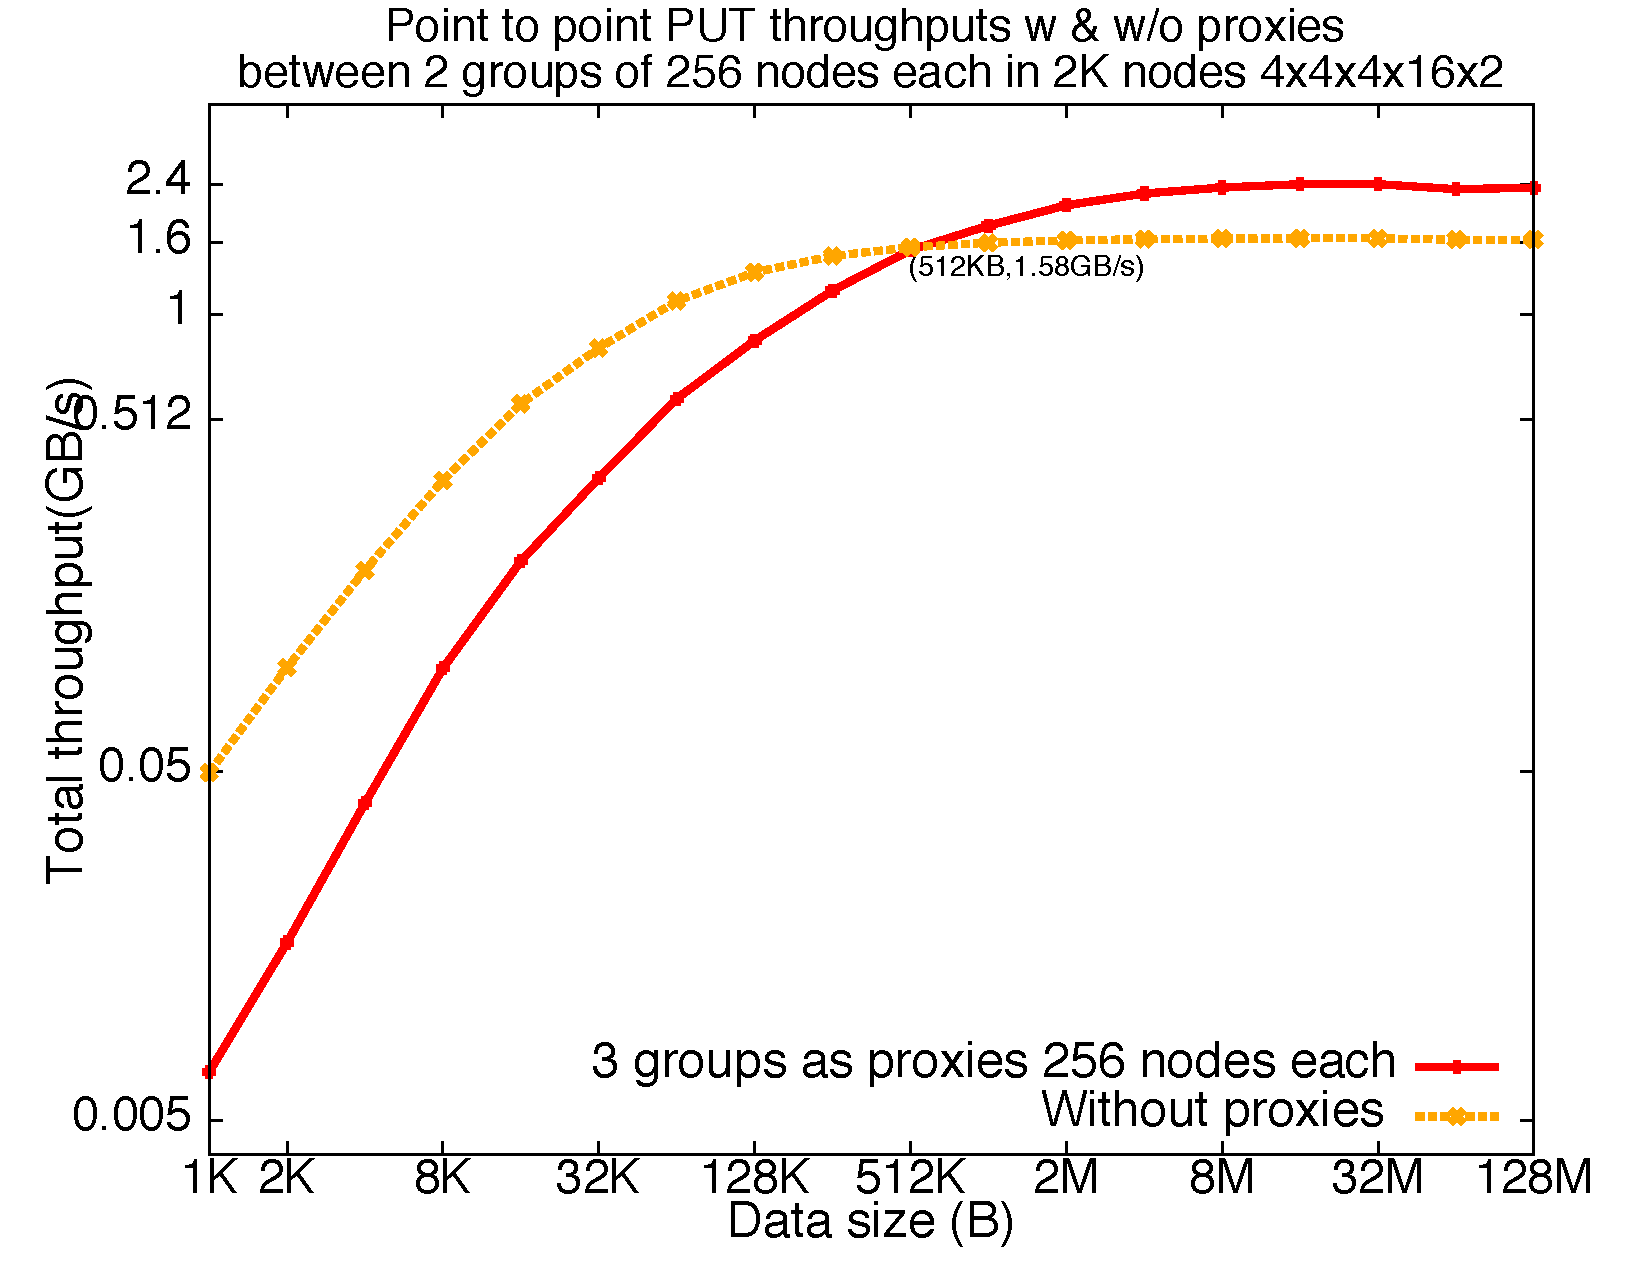
\includegraphics[scale=0.3]{figures/3groxies}
\vspace{-0.2in}
\caption{Using 3 group of proxies to improve data transfer bandwidth between 2 group of nodes}
\vspace{-0.1in}
\label{fig:3groxies}
\end{figure}

In the figure, we once again see that with small messages, direct transfer is better than proxy-based transfer. The threshold for this case increases to 512KB. At that message size, direct transfer also reaches to its maximum throughput, while the proxy-based transfer still has big room to increase up to 2.4GB/s. The performance increases $1.5\times$ as predicted since 3 proxies are used for each nodes. This benchmark shows that proxy-based data transfer is feasible for data transfer between groups of nodes. And we can achieve significant improvement in certain cases.

As we have mentioned in Section \ref{sec:approaches}, we need at least k $>$ 2 proxies per each data transfer to benefit from proxies. The more proxies we can use the better performance we can gain. However, as the size of communicating groups increases, the number of proxies we can set up decreases. If we add more proxies beyond the maximum possible proxies, data movements by extra proxies intervene existing ones and eventually degrade overall performance. The Figure \ref{fig:num_groxies} demonstrates the situation.

\begin{figure}[!htb]
\vspace{-0.1in}
\centering
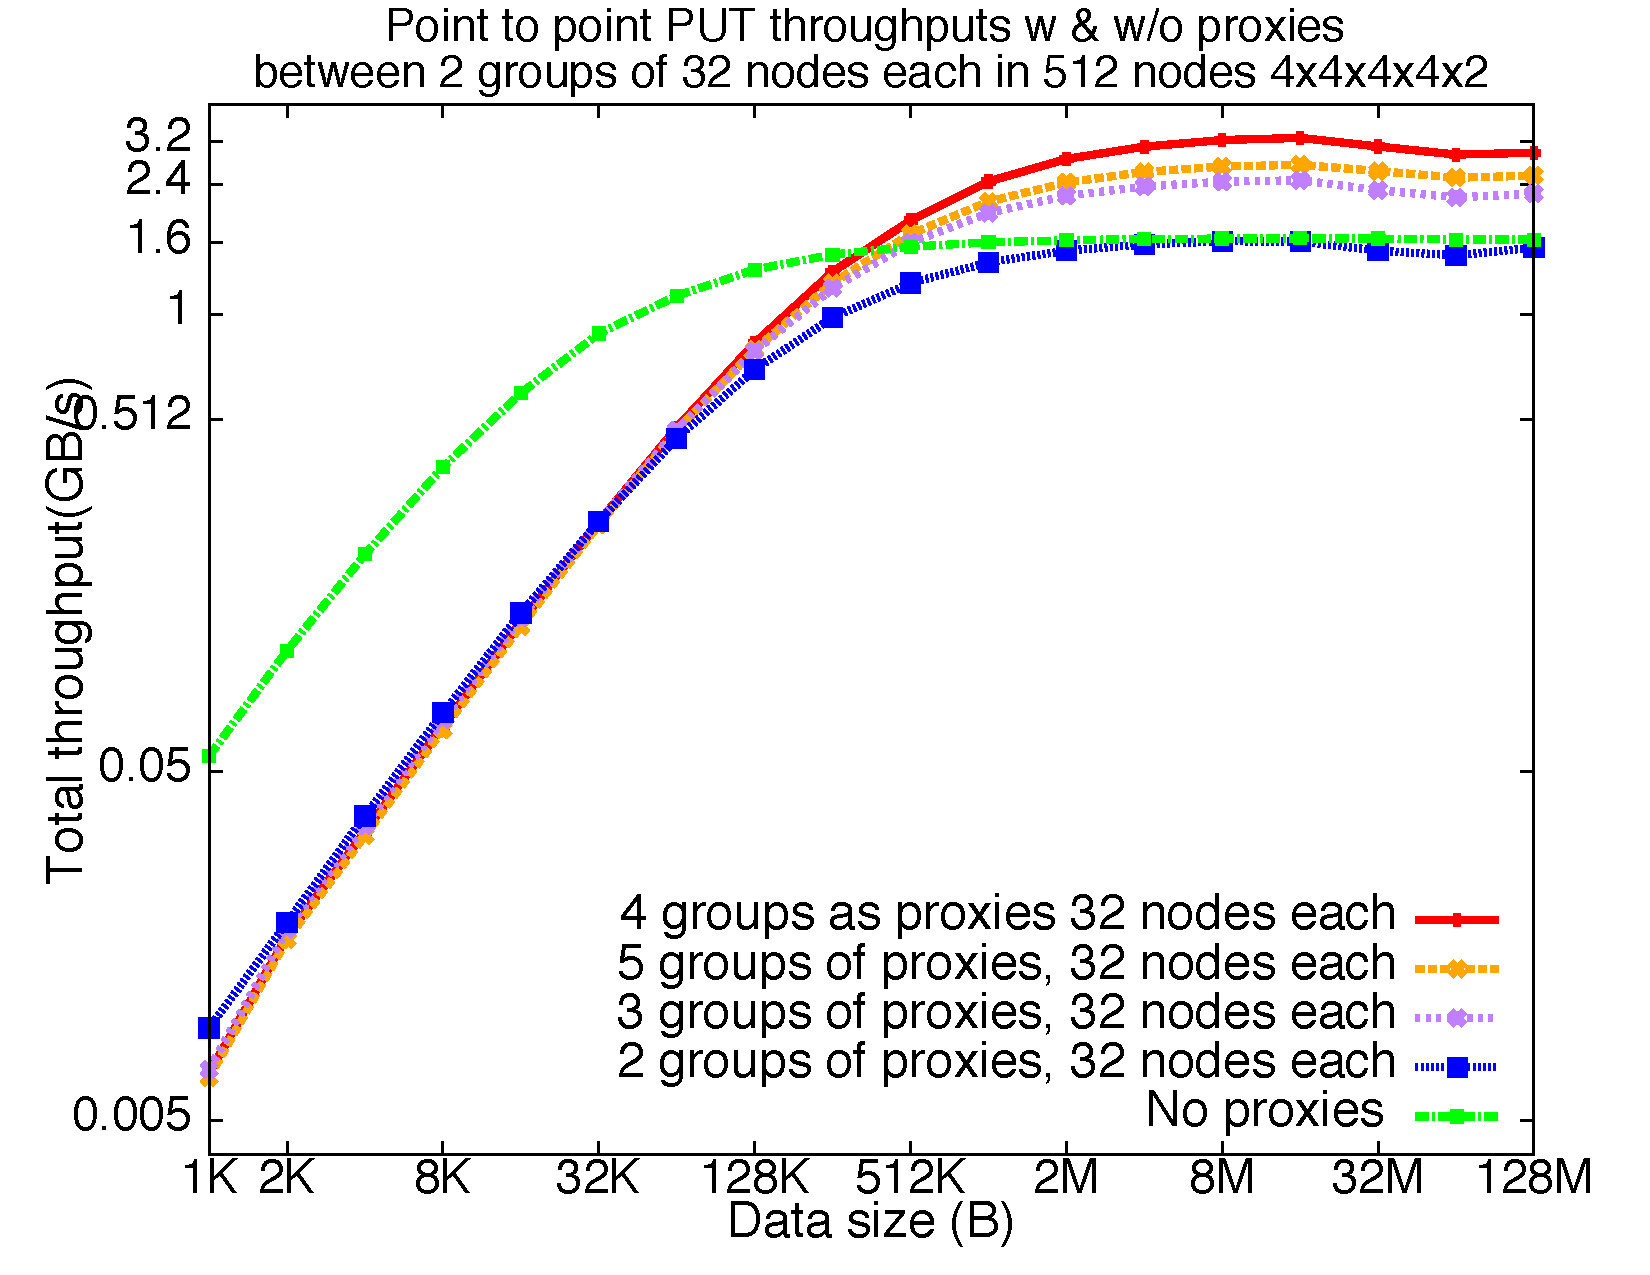
\includegraphics[scale=0.3]{figures/num_groxies}
\vspace{-0.2in}
\caption{Performance variance with number of proxies}
\label{fig:num_groxies}
\vspace{-0.1in}
\end{figure}

With the torus 4x4x4x4x2 and 2 groups of 32 nodes each, we can set up at most 4 groups of proxies along A+, A-, B+, B- dimensions. The 5th proxy is the source node itself. As Figure \ref{fig:num_groxies} shows, when we increases the number groups of proxies from 2 to 3 and to 4, the throughput increases from no-improvement, to 1.5$\times$ and to 2$\times$. Thus, with large message sizes, we can gain k/2 times performance with k being the number of proxies. However, when we increase number of proxies to 5, the performance starts to drop due to intervention among concurrent data movements. Therefore, choosing number of proxies together with their locations is important to maximize throughput.

The above three benchmarks demonstrate the efficaty of our solutions for data movement between compute nodes. In the next subsection, we evaluate our approaches in the case of data movement between compute nodes and I/O nodes. 

%\subsection{Sparse data patterns}


%In the next subsection, we present our benchmarks on the two data patterns generated.
%\subsection{Staging}

\subsection{Data Movement to I/O nodes}
We perform a weak scaling study with two sparse data patterns, and scale the number of cores from 2,048 to 131,072 cores on the Mira BG/Q system. 

\begin{itemize}
\item Pattern 1: Uniform distribution data where data size of a MPI rank is uniformly distributed between 0 and 8MB.  Data is generated by using \textit{srand()} and \textit{rand()} functions in C/C++ and using \textit{time(NULL)} as a seed.  Total data size is about 50\% of the dense data. The distribution of the data size is shown in Figure \ref{fig:uniform}.
\item Pattern 2: Pareto distribution data where many of MPI ranks have data size of 0 bytes or very low size, and a few of MPI ranks have data size of 8MB or close by. The total data size is about 20\% of the dense pattern. The distribution of the data is shown in Figure \ref{fig:pareto}
\end{itemize}

In the data pattern 1, data sizes are uniformly distributed among nodes. This data pattern can be seen when we want to analyze data from different regions with different resolutions. Depending on the resolution, data sizes may vary accordingly.

\begin{figure}[!htb]
\vspace{-0.2in}
\centering
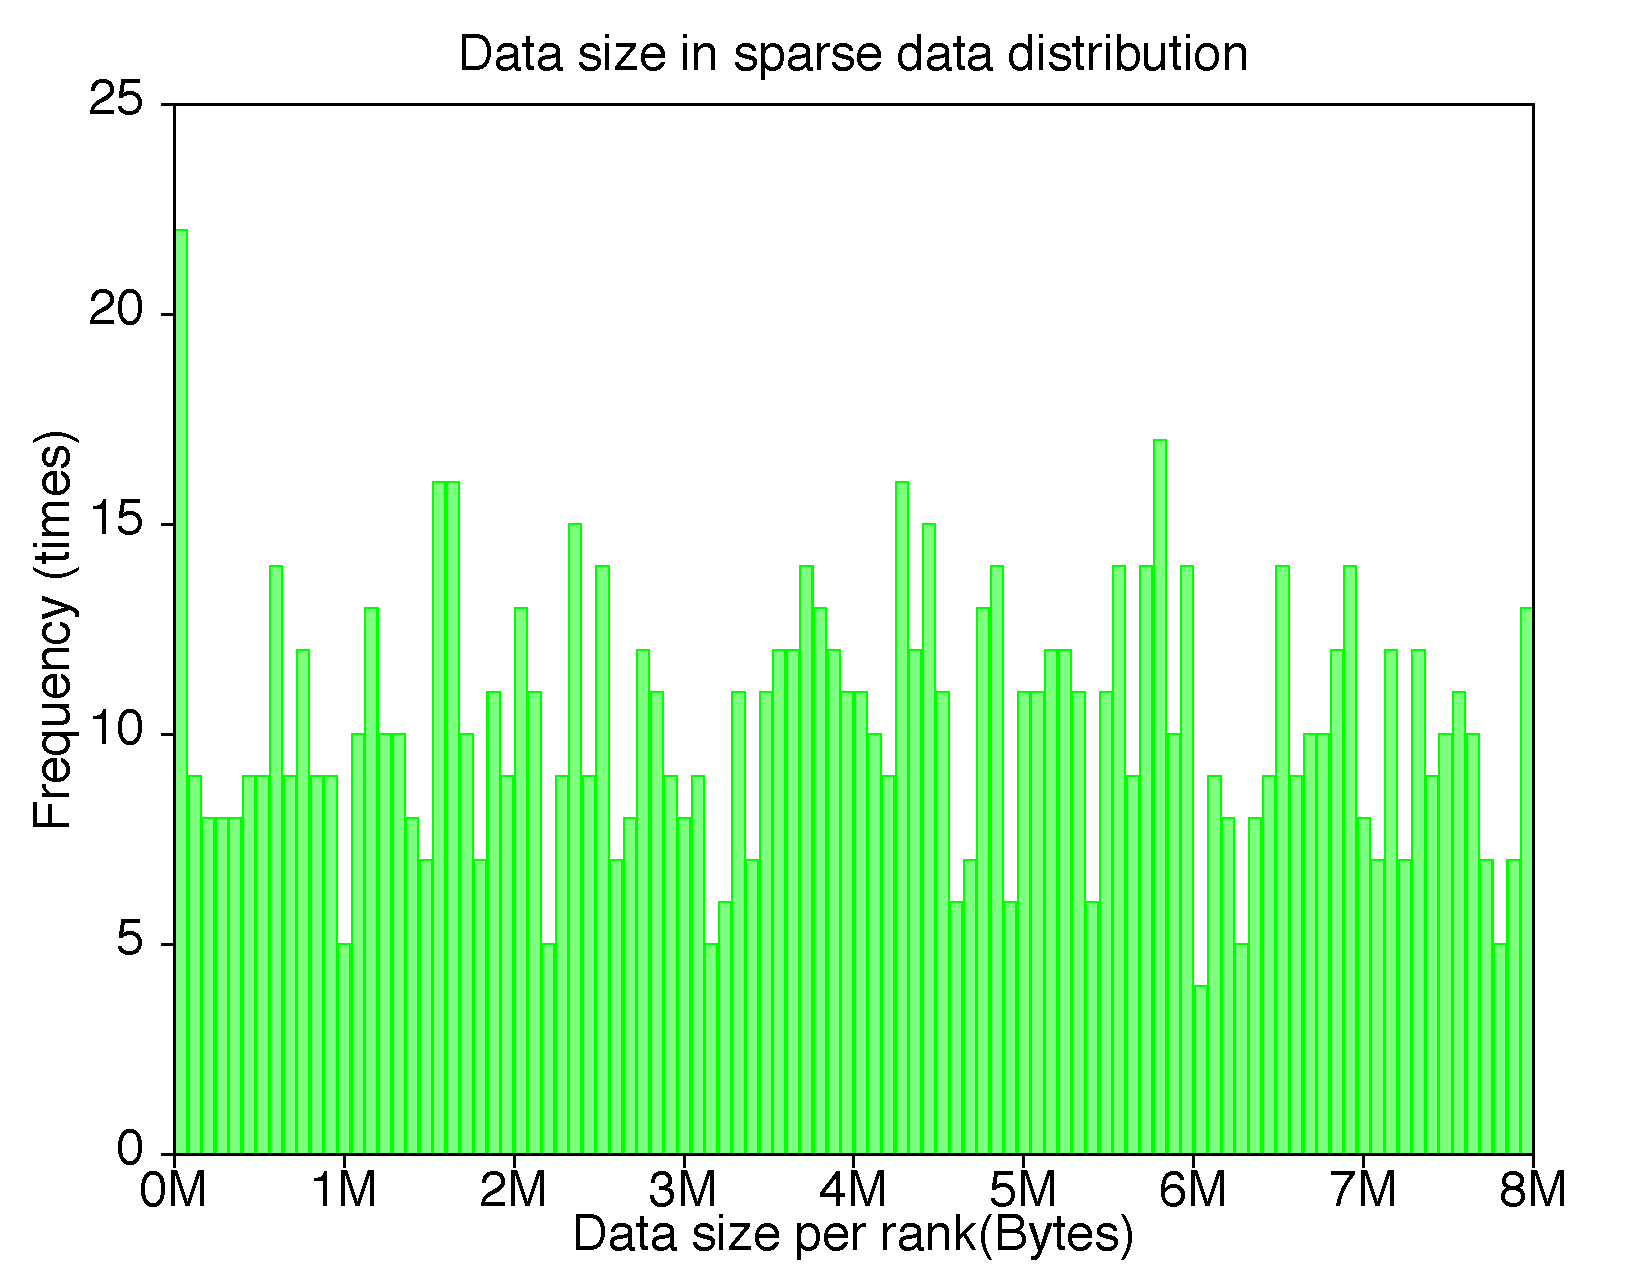
\includegraphics[scale=0.3]{figures/uniform.pdf}
\caption{Pattern 1: Histogram of data sizes for 1,024 processes using time(NULL) function with size from 0 to 8MB}
\label{fig:uniform}
\vspace{-0.1in}
\end{figure}

On the other hand, the data pattern 2 represents the case where data are sparse but not uniformly distributed. There are many nodes with almost no data while some nodes have large volume of data. This data pattern happens where we want to write out data from a region of contiguous MPI ranks while ignoring other regions.

\begin{figure}[!htb]
\vspace{-0.1in}
\centering
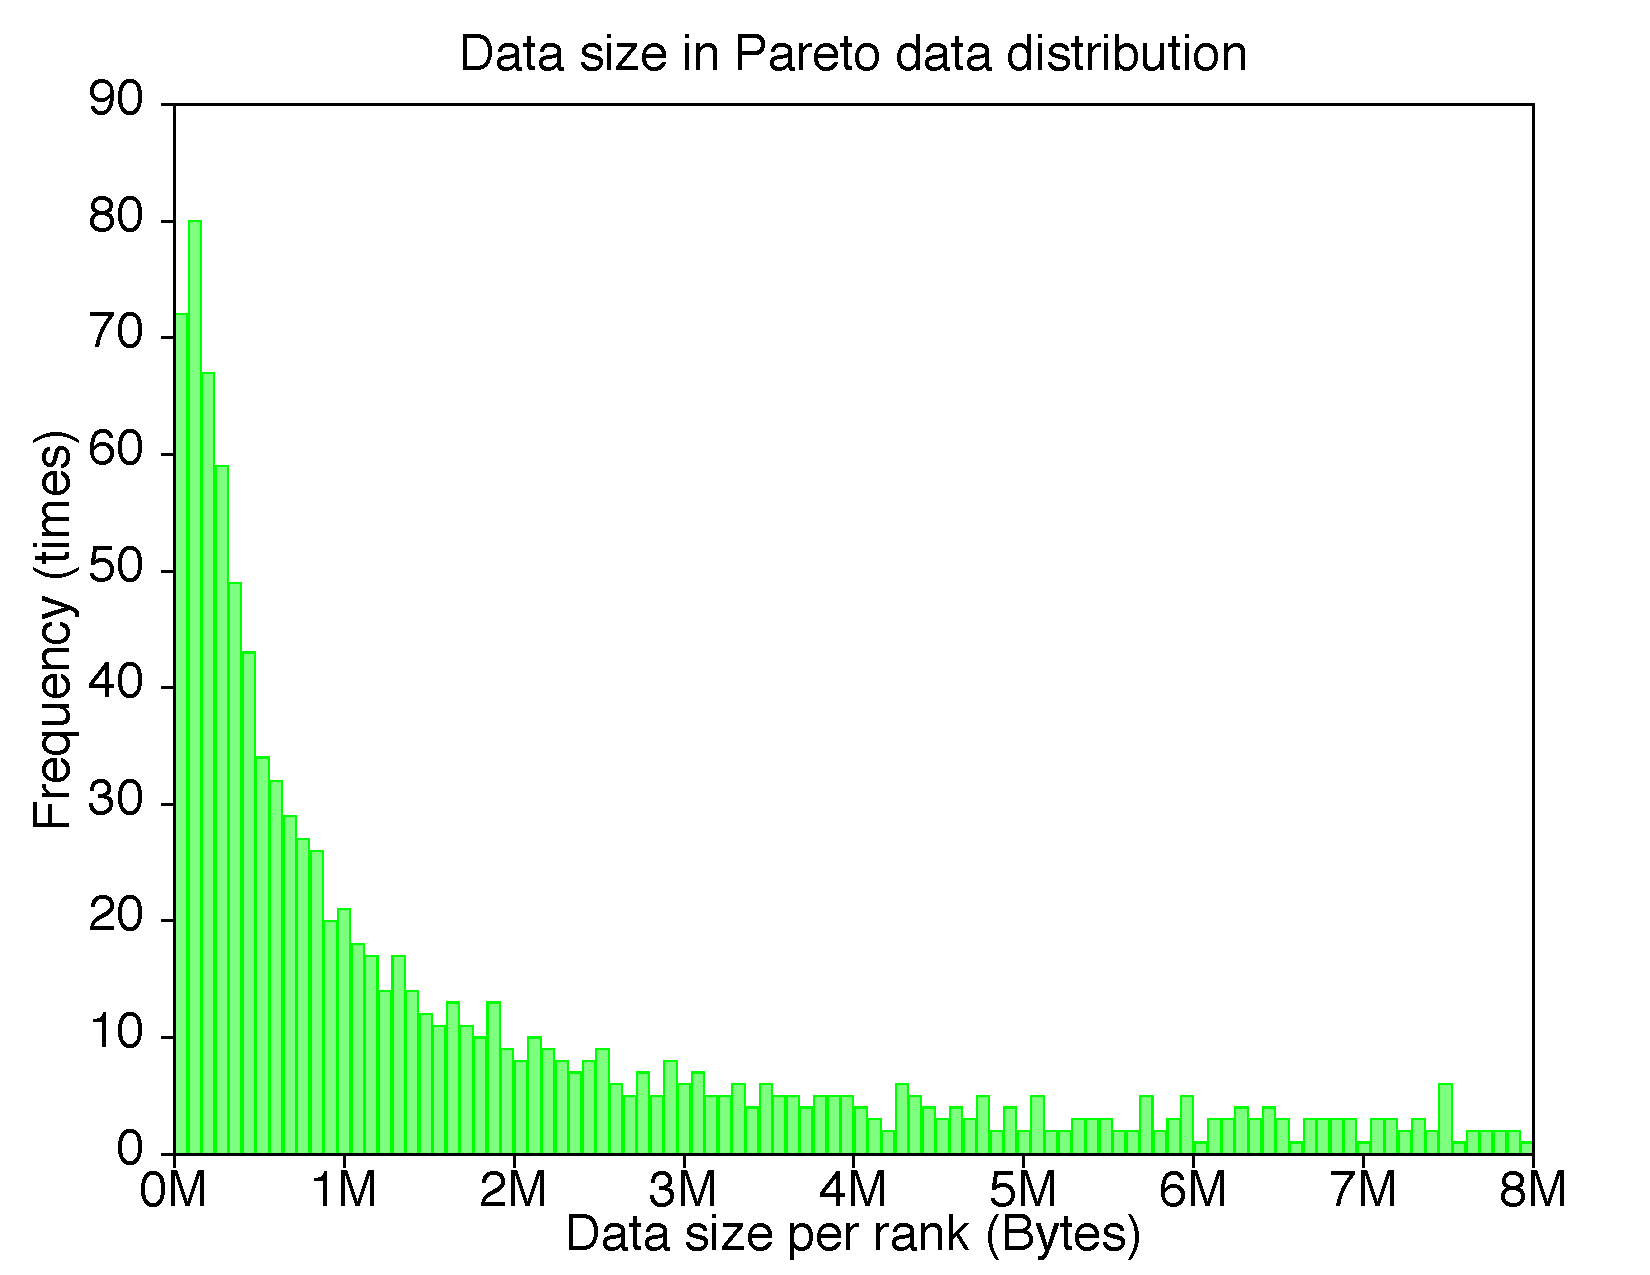
\includegraphics[scale=0.3]{figures/pareto.pdf}
\vspace{-0.1in}
\caption{Pattern 2: Histogram of data sizes of 1,024 processes using Pareto distribution function with size from 0B to 8MB}
\label{fig:pareto}
\vspace{-0.1in}
\end{figure}

On data pattern 1, we write roughly 8GB at 2,048 cores and 274GB of data at 131,072 cores. On data pattern 2, we write 3.4GB at 2,048 cores to 119GB of data at 131,072 cores. We compare the performance of performing aggregation for 2 data patterns using our approach and default MPI Collective I/O.

\begin{figure}[!htb]
\vspace{-0.1in}
\centering
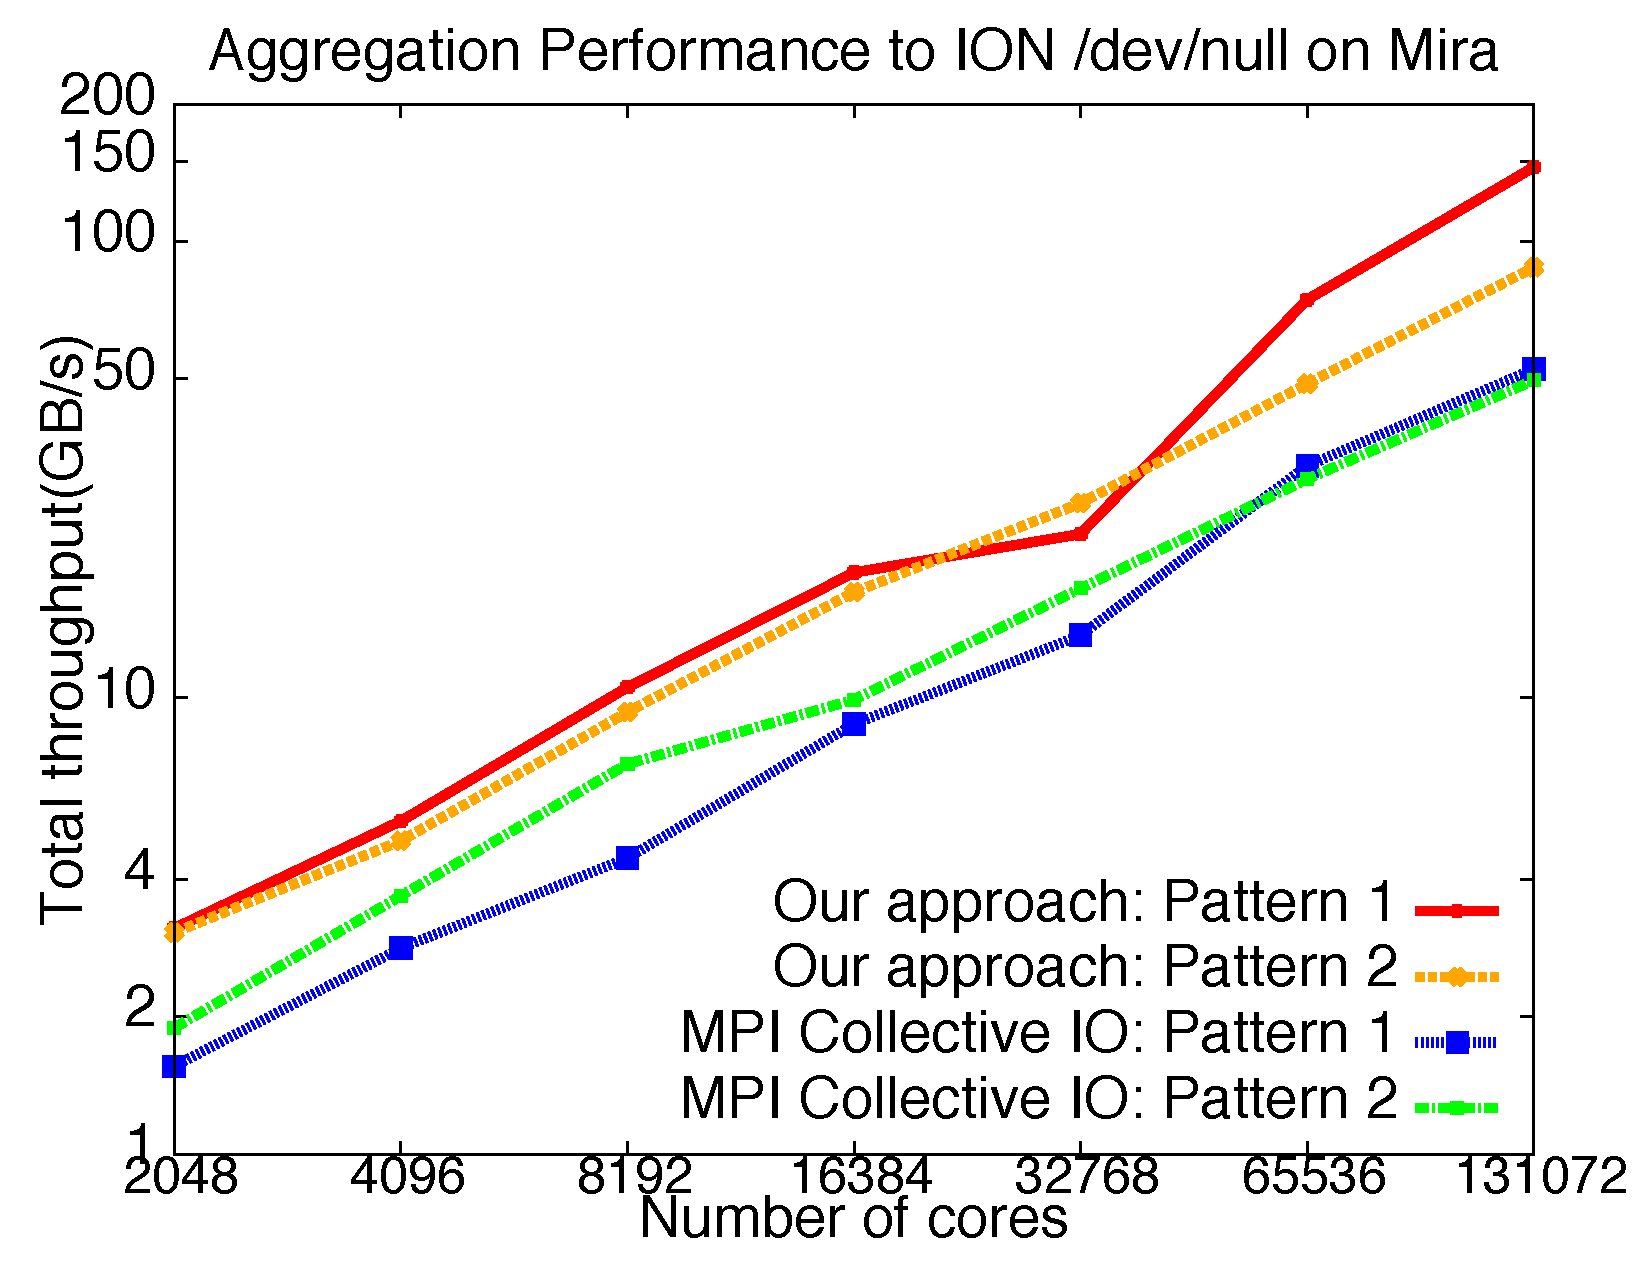
\includegraphics[scale=0.3]{figures/mira_agg.pdf}
\vspace{-0.2in}
\caption{Aggregation throughputs on Mira}
\vspace{-0.2in}
\label{fig:mira_agg}
\end{figure}

Figure \ref{fig:mira_agg} depicts the performance of our topology-aware multipath data movement approach in comparison to the default MPI-I/O for the two sparse data patterns as we scale from 2,048 cores to 131,072 cores on the Mira BG/Q system. On the data pattern 1 (uniformly distributed data), we observe  $2\times$ improvement at 2,048 cores. The performance increases as we scale and we achieve up to $3\times$ at 131,072 cores. On the data pattern 2 (pareto distributed data), we gain $1.5\times$ improvement at 2,048 cores and $2\times$ improvement at 131,072 cores. Thus, we observe that leveraging network interconnect topology and multipaths plays an important role at small scale and is critical at large scale. With the increased use of in-situ analysis for supercomputing,  sparse data patterns for I/O are becoming increasingly important and our approaches help provide more insights for improved performance.

\section{Application I/O benchmark}
\label{sec:app_benchmarks}
In this section, we demonstrate our solution on HACC I/O representing data movement between compute nodes and I/O nodes.

\subsection {HACC I/O}
HACC (Hardware/Hybrid Accelerated Cosmology Code) \cite{Habib:HACC} is a large-scale cosmology code suite that simulates the evolution of the universe through the first 13 billion years after the Big Bang. The simulation tracks the movement of trillions of particles as they collide and interact with each other, forming structure that transform into galaxies. During the runtime, HACC writes data periodically to storage system. The data can also be transferred from Mira to Tukey for data analysis and visualization. In both ways, data needs to go from compute nodes to I/O nodes first. In this benchmark, we use HACC I/O, an I/O benchmark written to evaluate performance of the I/O system for HACC, to show the data transfer performance from compute nodes to I/O nodes by writing to /dev/null. We compare the throughput of our mechanism to default MPI collective write on HACC I/O.
%\subsection{Staging}
%Presenting staging data from Mira to vis cluster Tukey. Analyze the results.

\subsection{Transferring data to I/O nodes}
In this experiments, we scale our experiments from 8,192 up to 131,072 compute cores to simulate the collision of $768^3$ to $2,816^3$ particles. We write only 10\% of the generated data with the amount of 2GB to 85GB of data. The data is written from processes with MPI ranks within the range [4*num\_processes/10, 5*num\_processes/10] with the num\_processes being the total number of MPI ranks in our application. We collect the bandwidth information and report the average. The results are shown in Figure \ref{fig:hacc_agg}

\begin{figure}[!htb]
\vspace{-0.1in}
\centering
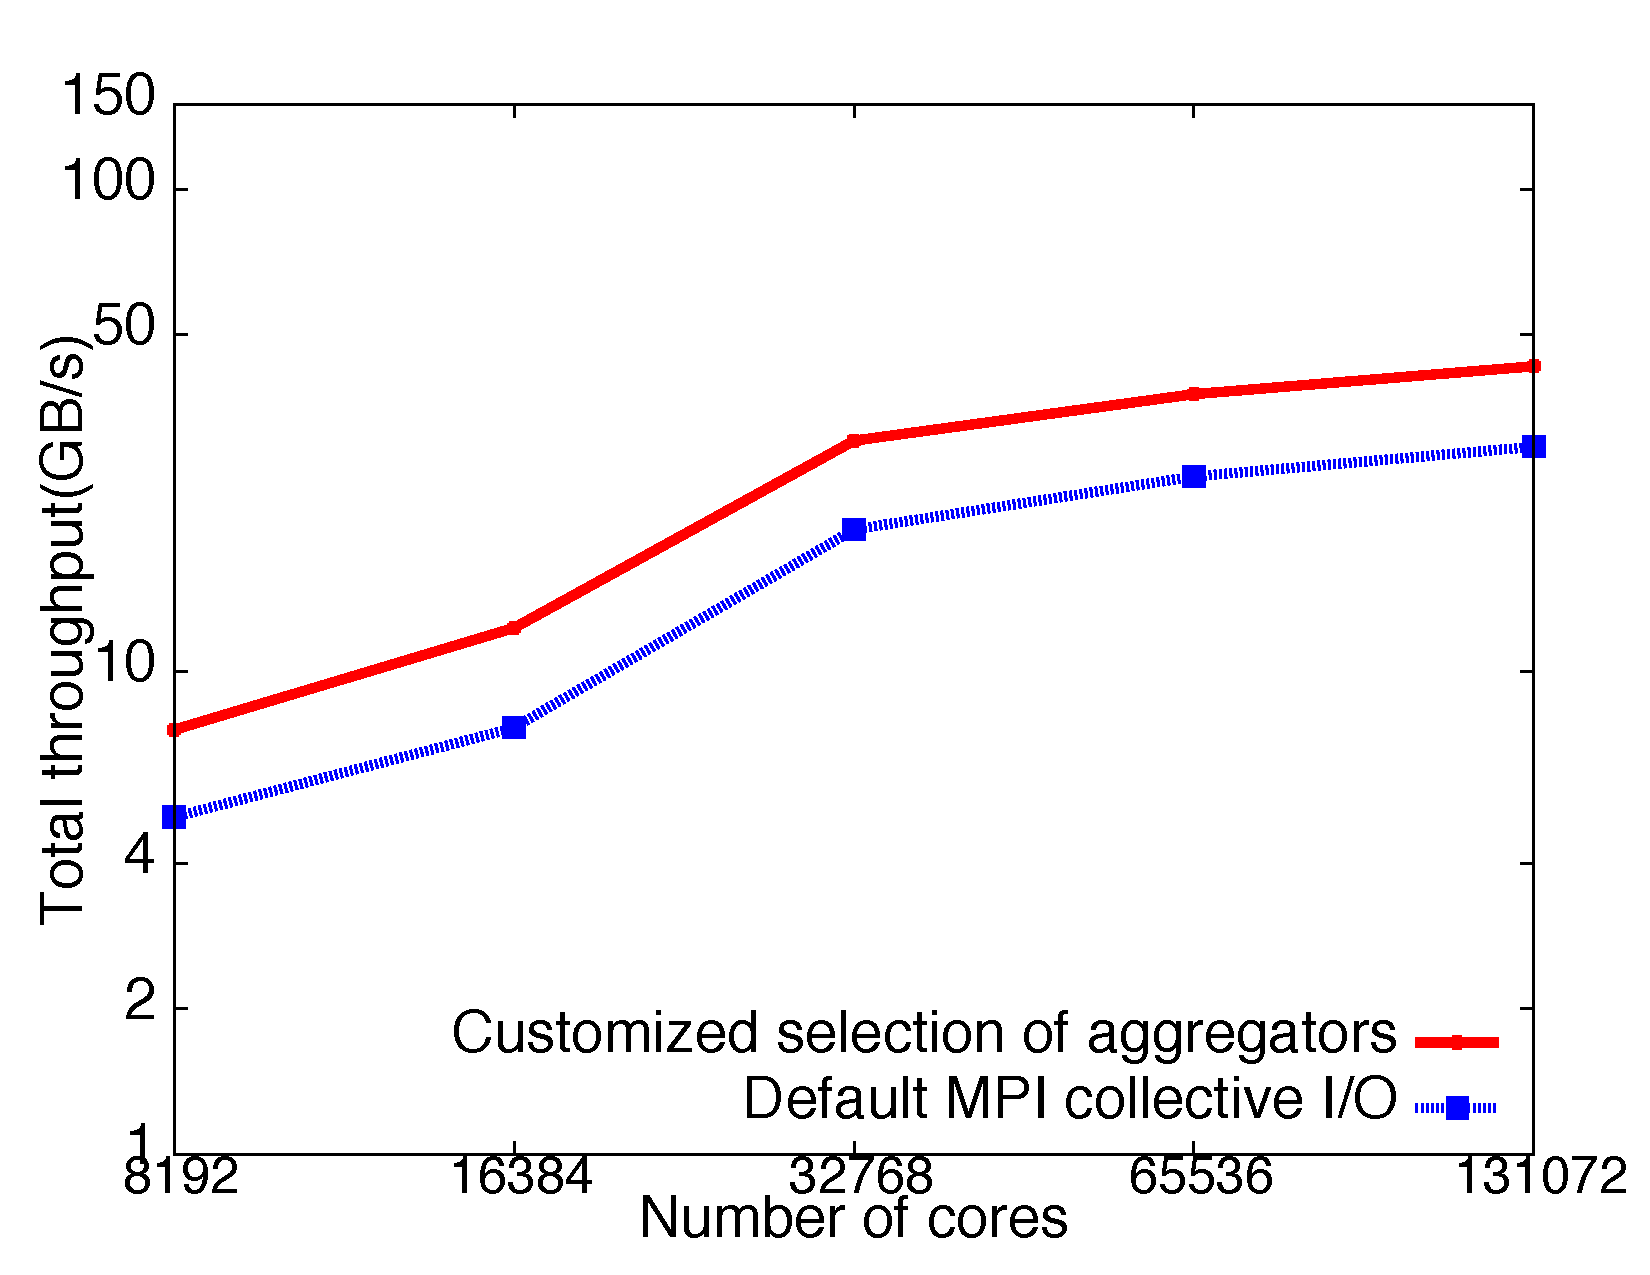
\includegraphics[scale=0.3]{figures/hacc_agg.pdf}
\vspace{-0.1in}
\caption{Write throughput of HACC application to I/O nodes /dev/null}
\vspace{-0.1in}
\label{fig:hacc_agg}
\end{figure}

The results show that in both cases, the number of I/O nodes employed is more than default I/O nodes. However, in our case, the position and location of aggregators are chosen dynamically and are distributed uniformly brought in better performance. Overall we can get up to 50\% throughput improvement. Thus, dynamic selection of number of and location of aggregators based on size of data and interconnect topology is of paramount importance for sparse data movement.

\subsection{Energy consumption comparison}
In these micro-benchmarks, we show that when using multi-path data movement for sparse data patterns, we not only increase bandwidth but also save energy consumption by the system.

\begin{figure}[!htb]
\vspace{-0.1in}
\centering
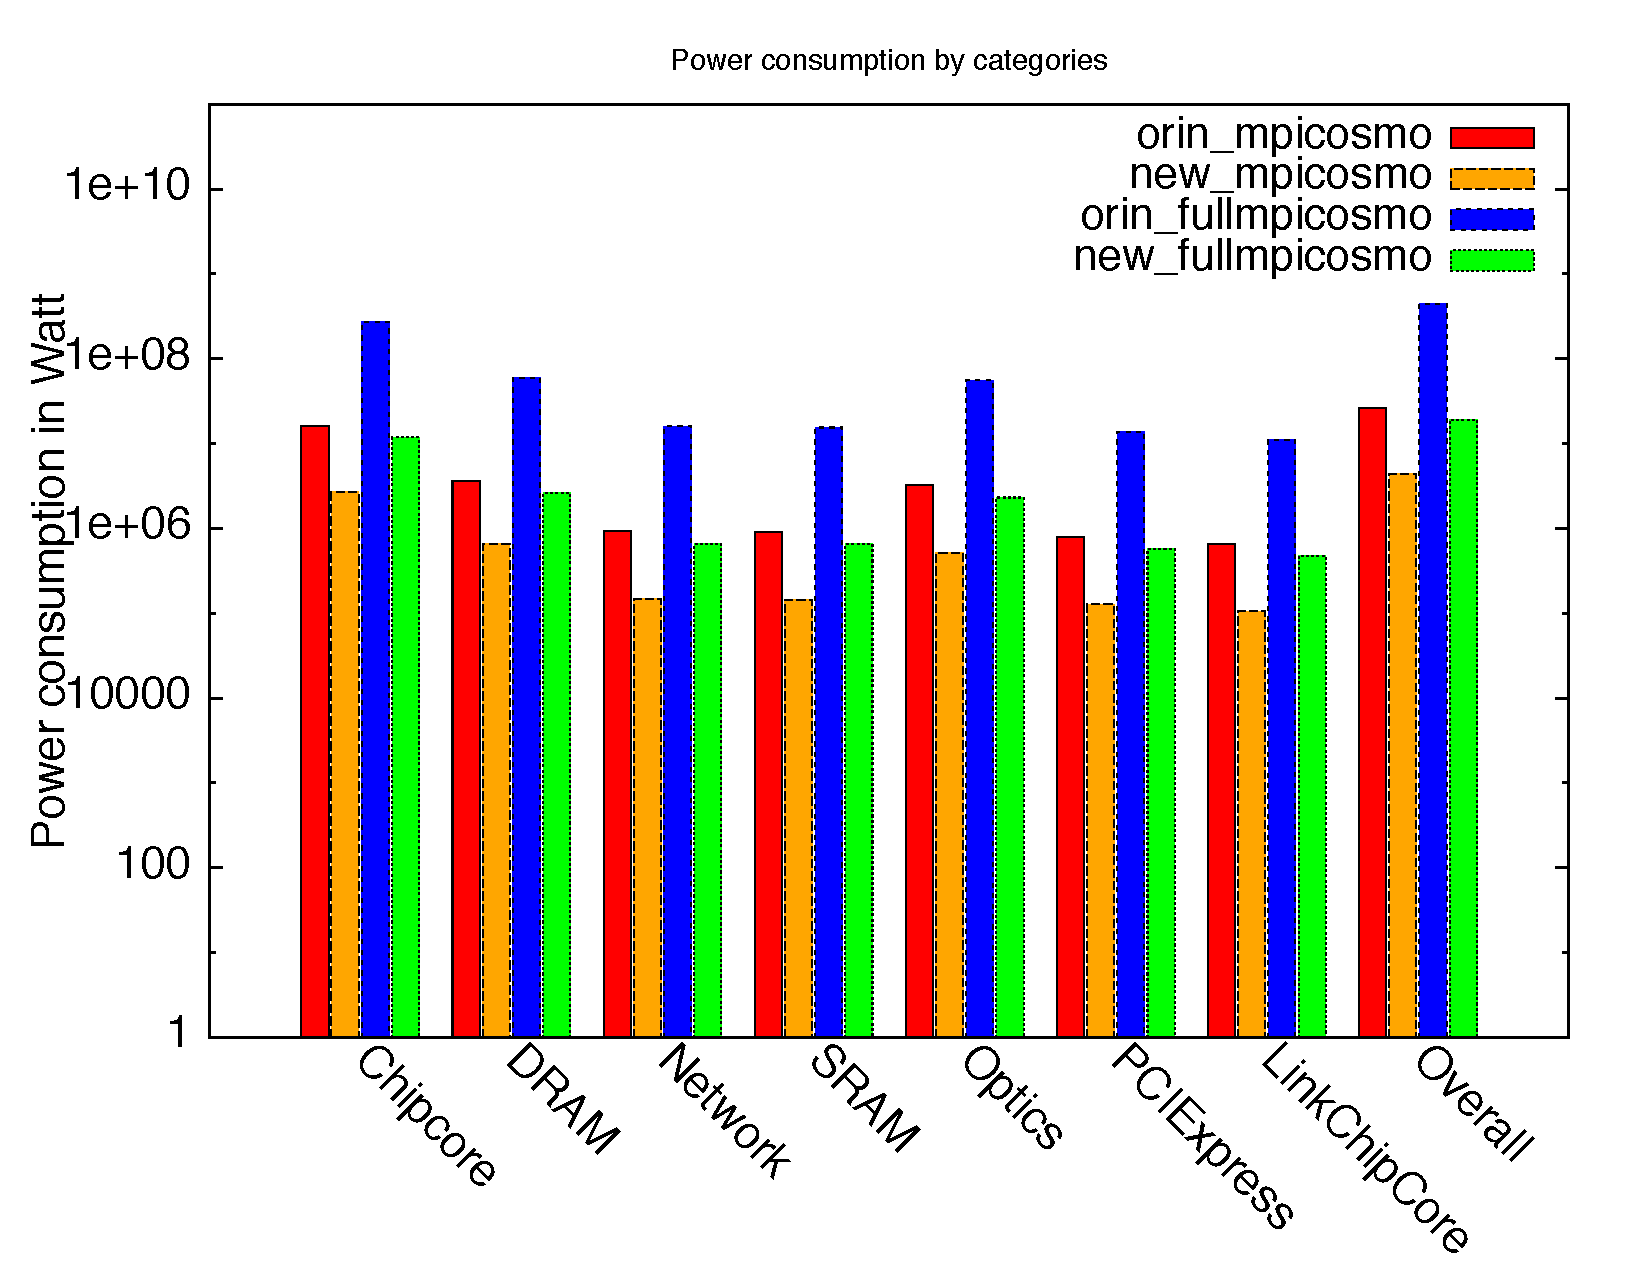
\includegraphics[scale=0.3]{figures/power_cat.pdf}
\vspace{-0.1in}
\caption{Energy consumption by category at a node}
\vspace{-0.1in}
\label{fig:hacc_agg}
\end{figure}

\begin{figure}[!htb]
\vspace{-0.1in}
\centering
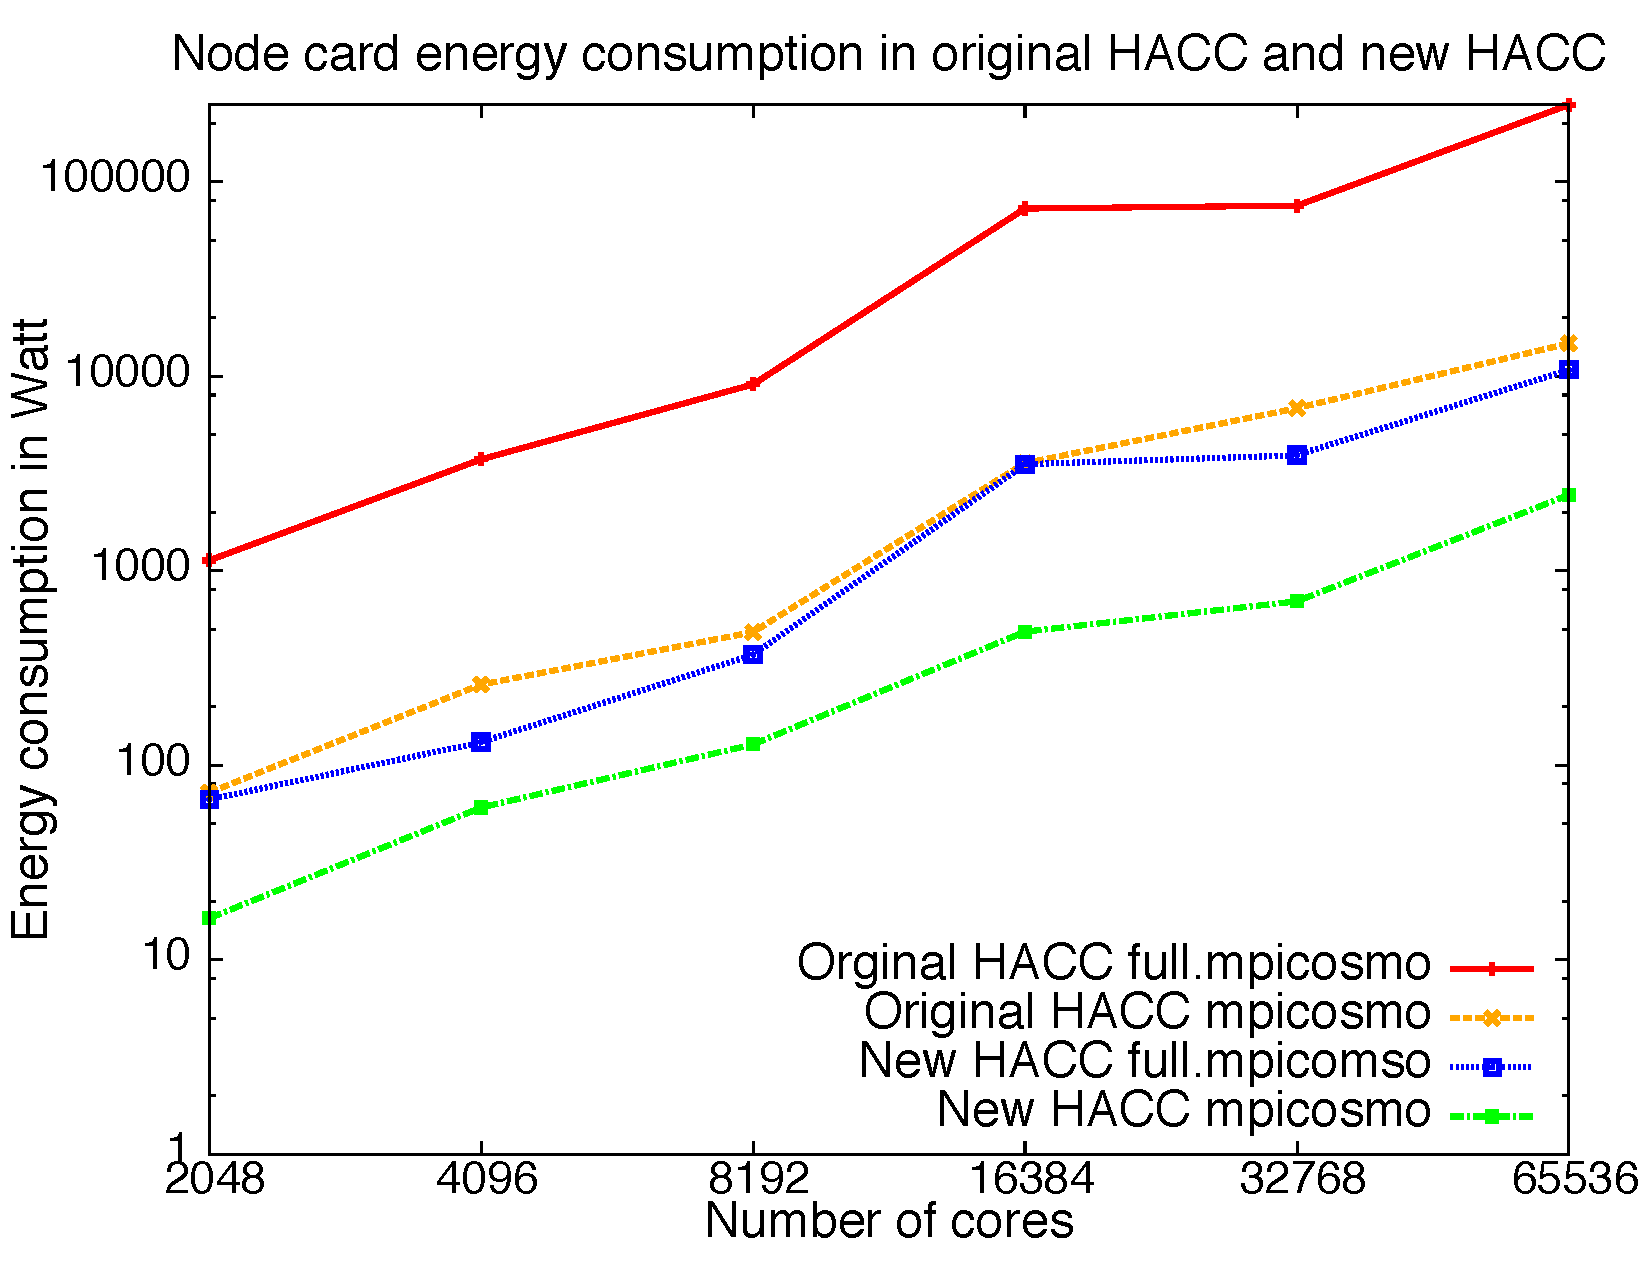
\includegraphics[scale=0.3]{figures/power_ncp.pdf}
\vspace{-0.1in}
\caption{Total energy consumption at scale}
\vspace{-0.1in}
\label{fig:hacc_agg}
\end{figure}

\section{Conclusions and future works}
\label{sec:conclusions}

In this paper, we present a scalable mechanism for improving sparse data movement, which often takes place in scientific applications such as  in-situ analysis and multiphysics applications, by utilizing underlying resources. Our approaches introduce intermediate nodes to increase data transfer throughput. Our solutions work for both sparse data movement between data coupling groups of nodes and sparse data movement between compute nodes and I/O nodes. We demonstrate the efficacy of our solutions through microbenchmarks and application benchmarks showing up to $2\times$ data movement throughput improvement. Our work shows that network topology aware data movement utilizing all available network resources helps improve the performance of data-intensive applications.
In the future, we plan to employ pipeline technique in which data will be split into small messages to be transferred. Thus, we will need only 2 proxies at least to get benefit from proxies-based method. We will come up with an analytical model for the achievable throughput and explore graph models for data movement in different network topologies and with different shapes of partitions given for physics modules.

\section*{Acknowledgments}

This research used resources of the Argonne Leadership Computing Facility (ALCF) at Argonne National Laboratory, and is supported by the Office of Science of the U.S. Department of Energy under contract DE-AC02-06CH11357. We thank the ALCF team for discussions and help related to this paper.

%% The Appendices part is started with the command \appendix;
%% appendix sections are then done as normal sections
%% \appendix

%% \section{}
%% \label{}

\section*{References}

%% If you have bibdatabase file and want bibtex to generate the
%% bibitems, please use
%%
\bibliographystyle{elsarticle-num} 
\bibliography{sigproc}

%% else use the following coding to input the bibitems directly in the
%% TeX file.

%\begin{thebibliography}{00}

%% \bibitem{label}
%% Text of bibliographic item

%% \bibitem{}

%\end{thebibliography}
\end{document}
\endinput
%%
%% End of file `elsarticle-template-num.tex'.
